%%
%% This is file `sample-manuscript.tex',
%% generated with the docstrip utility.
%%
%% The original source files were:
%%
%% samples.dtx  (with options: `manuscript')
%%
%% IMPORTANT NOTICE:
%%
%% For the copyright see the source file.
%%
%% Any modified versions of this file must be renamed
%% with new filenames distinct from sample-manuscript.tex.
%%
%% For distribution of the original source see the terms
%% for copying and modification in the file samples.dtx.
%%
%% This generated file may be distributed as long as the
%% original source files, as listed above, are part of the
%% same distribution. (The sources need not necessarily be
%% in the same archive or directory.)
%%
%% The first command in your LaTeX source must be the \documentclass command.
%%%% Small single column format, used for CIE, CSUR, DTRAP, JACM, JDIQ, JEA, JERIC, JETC, PACMCGIT, TAAS, TACCESS, TACO, TALG, TALLIP (formerly TALIP), TCPS, TDSCI, TEAC, TECS, TELO, THRI, TIIS, TIOT, TISSEC, TIST, TKDD, TMIS, TOCE, TOCHI, TOCL, TOCS, TOCT, TODAES, TODS, TOIS, TOIT, TOMACS, TOMM (formerly TOMCCAP), TOMPECS, TOMS, TOPC, TOPLAS, TOPS, TOS, TOSEM, TOSN, TQC, TRETS, TSAS, TSC, TSLP, TWEB.
% \documentclass[acmsmall]{acmart}

%%%% Large single column format, used for IMWUT, JOCCH, PACMPL, POMACS, TAP, PACMHCI
% \documentclass[acmlarge,screen]{acmart}

%%%% Large double column format, used for TOG
% \documentclass[acmtog, authorversion]{acmart}

%%%% Generic manuscript mode, required for submission
%%%% and peer review
\documentclass[sigconf, review, anonymous]{acmart}
\usepackage{balance}
\usepackage{amsthm}
\usepackage{hyperref}
\usepackage{algorithm}
\usepackage[noend]{algpseudocode}
%% Fonts used in the template cannot be substituted; margin
%% adjustments are not allowed.
%%
%% \BibTeX command to typeset BibTeX logo in the docs
\AtBeginDocument{%
  \providecommand\BibTeX{{%
    \normalfont B\kern-0.5em{\scshape i\kern-0.25em b}\kern-0.8em\TeX}}}

%% Rights management information.  This information is sent to you
%% when you complete the rights form.  These commands have SAMPLE
%% values in them; it is your responsibility as an author to replace
%% the commands and values with those provided to you when you
%% complete the rights form.
\setcopyright{acmcopyright}
\copyrightyear{2021}
\acmYear{2021}
\acmDOI{10.1145/1122445.1122456}

%% These commands are for a PROCEEDINGS abstract or paper.
\acmConference[NSPW 2021]{NSPW: New Security Paradigms Workshop}
{October 25--28, 2021}{North Conway, NH}
\acmBooktitle{NSPW '21: New Security Paradigms Workshop,
  October 25--28, 2021,North Conway, NH}
\acmPrice{15.00}
\acmISBN{978-1-4503-XXXX-X/18/06}


%%
%% Submission ID.
%% Use this when submitting an article to a sponsored event. You'll
%% receive a unique submission ID from the organizers
%% of the event, and this ID should be used as the parameter to this command.
%%\acmSubmissionID{123-A56-BU3}

%%
%% The majority of ACM publications use numbered citations and
%% references.  The command \citestyle{authoryear} switches to the
%% "author year" style.
%%
%% If you are preparing content for an event
%% sponsored by ACM SIGGRAPH, you must use the "author year" style of
%% citations and references.
%% Uncommenting
%% the next command will enable that style.
%%\citestyle{acmauthoryear}

%%
%% end of the preamble, start of the body of the document source.
\newtheoremstyle{mydef}
{\topsep}{\topsep}%
{}{}%
{\bfseries}{}
{\newline}
{%
  \rule{.48\textwidth}{0.4pt}\\*%
  \thmname{#1}~\thmnumber{#2}\thmnote{\ -\ #3}.\\*[-1.5ex]%
  \rule{.48\textwidth}{0.4pt}}%

\theoremstyle{mydef}

\newtheorem{definition}{Definition}

\begin{document}

%%
%% The "title" command has an optional parameter,
%% allowing the author to define a "short title" to be used in page headers.
\title{COLBAC: Shifting Cybersecurity from Hierarchical to Horizontal designs}

%%
%% The "author" command and its associated commands are used to define
%% the authors and their affiliations.
%% Of note is the shared affiliation of the first two authors, and the
%% "authornote" and "authornotemark" commands
%% used to denote shared contribution to the research.
\author{Kevin Gallagher}
%\authornote{Both authors contributed equally to this research.}
\email{kevin.gallagher@nyu.edu}
%\orcid{1234-5678-9012}
\affiliation{%
    \institution{Department Of Computer Science and Engineering\\New York University}
    \streetaddress{370 Jay Street, 10th Floor}
    \city{Brooklyn}
    \state{New York}
    \country{USA}
    \postcode{11021}
}
\email{kevin.gallagher@privacylx.org}
\affiliation{%
    \institution{Defend Our Privacy Association (PrivacyLX)}
    %\city{Lisboa}
    \state{Lisboa}
    \country{Portugal}
}

\author{Jessica Feldman}
\email{jfeldman@aup.edu}
%\orcid{1234-5678-9012}
\affiliation{%
    \institution{Department of Communication, Media, and Culture\\ American University of Paris}
    \streetaddress{5, Boulevard de La Tour-Maubourg}
    \city{Paris}
    %\state{}
    \country{France}
    \postcode{75007}
}

\author{Santiago Torres-Arias}
\email{santiagotorres@purdue.edu}
\affiliation{
    \institution{Department of Electrical and Computer Engineering\\ Purdue University}
    \streetaddress{501 Northwestern Avenue}
    \city{Wast Lafayette}
    \state{Indiana}
    \country{United States of America}
    \postcode{47907-2305}
}

\author{Nasir Memon}
\email{memon@nyu.edu}
\affiliation{
    \institution{Department of Computer Science and Engineering\\ New York University}
    \streetaddress{370 Jay Street, 10th floor}
    \city{Brooklyn}
    \state{New York}
    \country{United States of America}
    \postcode{11201}
}

%%
%% By default, the full list of authors will be used in the page
%% headers. Often, this list is too long, and will overlap
%% other information printed in the page headers. This command allows
%% the author to define a more concise list
%% of authors' names for this purpose.
\renewcommand{\shortauthors}{Gallagher, Feldman, and Torres}

%%
%% The abstract is a short summary of the work to be presented in the
%% article.
\begin{abstract}
Cybersecurity suffers from an oversaturation of centralized, hierarchical
systems and a lack of exploration in the area of horizontal security, or
security techniques and technologies which utilize democratic participation for
security decision-making. Because of this, many horizontally governed
organizations such as activist groups, worker cooperatives, trade unions,
not-for-profit associations, and others are not represented in current
cybersecurity solutions, and are forced to adopt hierarchical solutions to
cybersecurity problems. This causes power dynamic mismatches that lead to
cybersecurity and organizational operations failures. In this work we introduce
COLBAC, a collective based access control system aimed at addressing this lack.
COLBAC uses democratically authorized capability tokens to express access
control policies. It allows for a flexible and dynamic degree of horizontality
to meet the needs of different horizontally governed organizations. After
introducing COLBAC, we finish with a discussion on future work needed to realize
more horizontal security techniques, tools, and technologies.

\end{abstract}

%%
%% The code below is generated by the tool at http://dl.acm.org/ccs.cfm.
%% Please copy and paste the code instead of the example below.
%%

\begin{CCSXML}
<ccs2012>
   <concept>
       <concept_id>10002978.10002991.10002993</concept_id>
       <concept_desc>Security and privacy~Access control</concept_desc>
       <concept_significance>300</concept_significance>
       </concept>
   <concept>
       <concept_id>10002978.10002991.10010839</concept_id>
       <concept_desc>Security and privacy~Authorization</concept_desc>
       <concept_significance>500</concept_significance>
       </concept>
   <concept>
       <concept_id>10002978.10003029.10011703</concept_id>
       <concept_desc>Security and privacy~Usability in security and privacy</concept_desc>
       <concept_significance>500</concept_significance>
       </concept>
   <concept>
       <concept_id>10002978.10003029.10003032</concept_id>
       <concept_desc>Security and privacy~Social aspects of security and privacy</concept_desc>
       <concept_significance>500</concept_significance>
       </concept>
 </ccs2012>
\end{CCSXML}

\ccsdesc[300]{Security and privacy~Access control}
\ccsdesc[500]{Security and privacy~Authorization}
\ccsdesc[500]{Security and privacy~Usability in security and privacy}
\ccsdesc[500]{Security and privacy~Social aspects of security and privacy}

%%
%% Keywords. The author(s) should pick words that accurately describe
%% the work being presented. Separate the keywords with commas.
\keywords{security, democracy, activism, horizontality, participation, participatory design, distributed systems, authorization, access control}

\maketitle

\section*{Justification Statement}
\label{sec:justification}
In this work we challenge the existing hierarchical approaches to access control
and provide an alternative system for horizontal and participatory access
control. We believe that this work fits as a regular submission to NSPW since it
recognizes the limitations of an existing security paradigm and proposes a new
solution that solves the problem of access control in a more fair, horizontal,
and participatory way. To our knowledge there is no other access control system
that attempts this, making this a novel angle to approach access control. Since
access control is a security primitive that other security systems are built on
top of, the introduction of a horizontal method of access control may open up
new possibilities for re-envisioning security tools and techniques.


\section{Introduction}
\label{sec:introduction}
Recent events all around the globe have demonstrated an increasing desire for
more inclusive, participatory, and fair social structures. From the demands of
Black Lives Matter protesters regarding police oversight and funding, to the
popular reactions to the handling of the COVID pandemic, to the decision making
power over the product of a worker's labor, people are continuing to demand more
participation in important economic and societal decision-making processes. %TODO: CITE ME
Even some schools are beginning to include the democratic participation of the
school children to their decision making processes, encouraging engagement and
investment in the child's own education.~\cite{pacheco2008escola}

This shift in organization has potential implications in how organizations
interact internally, with each other, and with society as a whole. Whereas the
interactions between a hierarchical organizations are overwhelmingly guided by
the visions of the individuals who are on top of their respective organization's
hierarchies, interactions of more horizontal organizations are more complex, and
are meant to reflect the will of the entire group that make up the organization.
In addition, responsibilities in more horizontal organizations tend to shift.
For example, in worker cooperatives individuals often shift between different
job positions in order to learn how the company as a whole functions, and to
keep their work fresh and 
interesting~\cite{jackall19846, wright2014worker, lindenfeld1982workplace}.
To complicate matters further, different organizations have different, and
sometimes dynamic, levels of  horizontality~\cite{wright2014worker}. Some decide
to shift all decision making power to the collective, making approval for all
important actions require democratic votes or consensus. Others select
representatives or working groups to delegate specific tasks, allowing for
quicker actions and responses to events, but within a power structure that
allows for the revocation of those who misuse their power. Some organizations
take a hybrid approach, requiring democratic votes of the whole organization for
some issues, and electing working groups for others.

Despite the rapid demand of this changed structure of organization, 
Cybersecurity tools, technologies and techniques continue to remain highly 
hierarchical. Security policies are written by a security team or imported from
pre-existing (and sometimes external) templates and imposed on the rest of the
organization, with at most the limited oversight and approval of a manager or
higher-up. Even still, not every member of the security teams are participating
in deciding what these policies are meant to achieve. This decision is often
made by a manager, who ensures that the policies do not get in the way of the
visions of the individuals in the chief officer positions. {\color{red}TODO: CITE ME} These technologies
and policies reflect political decisions made during the creation of these
processes and technologies, and the technologies and policies themselves have
political implications~\cite{winner1980artifacts}.

More, secrets such as organizational passwords to third-party services are often
trusted to one individual or small group in an organization, but easily
recovered by an administrator or other individual higher in the hierarchy in the
case that the individual responsible leaves the organization or performs a
violation. However, when an organization becomes less hierarchical, the decision
of who should have access to such secrets becomes more difficult to make. If
everyone should have access to the secrets, such as passwords, then any insider
can change the passwords and cause denial of service for the organization. If
only a few people have the password, then a natural hierarchy forms based on
one's access to confidential organizational material. As Kavada states,
administrators hold great power over their respective
organizations~\cite{kavada2020counterpublics}.

\begin{quotation}
\textit{Yet, the material design and regulation of social media platforms soon
put anonymous administrators into leadership positions. In both movements,
social media gave the administrators a public stage to distribute messages to
large numbers of people and exclusive access to the metrics and demographics of
user engagement. On Facebook pages, for instance, admin posts are displayed on
the main timeline and are directly visible to users. On large pages... user
comments are... like a continuous stream with the admin post as the frame. Admin
posts are also written in a collective voice since administrators speak as [the
collective]. This provides administrators with significant power as they can
embody the collective voice of the movement.}
\end{quotation}

Kavada then discusses the concept of a ``password war,'' or a series of
interactions in which administrators of groups attempt to lock each other out of
the group social media page by changing passwords. This may harm the perceived
legitimacy of the movements, since one may believe that it represents that the
organization cannot achieve its own ideals.

This design issue also leads to the ``digital vanguard'' problem outlined by
Paulo Gerbaudo: in so-called ``leaderless'' social movements, those participants
who take on the role of managing the communications platforms end up taking on a
``vanguard'' role insofar as they are able to set the tone and agenda of the
movement through these communications.{\color{red} TODO: Cite me} Gerbaudo’s, Kavada's, and other % will change to our own after reviews. It gives a hint to who is authoring the work.
ethnographic research confirms that bitter struggles have occurred in many of
these nonhierarchical social movements and democratic political groups over 
control of passwords and administration of platforms, sometimes accelerating to
the point of lawsuits.

However, this may not be the fault of the organization itself. How can an 
organization achieve the goals of horizontality and equality when the tools they
must use for organization assume hierarchy, and grant some individuals more
control than others? Must these tools be this way? Are there better ways to
design tools to account for horizontality and equality in a client organization?
If a tool does not allow for horizontality and equality in a client
organization, can another tool sit in between the offending tool and the
organization to address the issue? In his work \textit{The Moral Character of
Cryptographic Work}, Rogaway states ``Cryptography can be developed in
directions that tend to benefit the weak \textit{or} the 
powerful.''~\cite{rogaway2015moral}. Why, then, have we not developed technology
that benefits the community of powerless by limiting the privileges of the
powerful within an organization via democratic vote?

In this paper we define and argue for the construction of horizontal security.
We explore different potential approaches to horizontal security, and examine
some examples of horizontal security practices currently in use. We then address
some potential benefits and drawbacks of horizontal security, and the effects it
may have on privacy. We then conclude with future work, and supply a set of
unsolved problems that must be addressed to realize our vision of horizontal
security.


\section{Envisioning Horizontal Security}
\label{sec:envisioning}
% In order to understand the concept of horizontal security, we must first examine
% the current state of security and its goals. For the purposes of this work, we
% will examine security through the traditional scheme of Confidentiality,
% Integrity and Availability.

% XXX: I'd like to flip "individual' to entity, as it feels that we could be
% talking about bots/platforms/processes and more in this horizontal security
% fashion
% XXX: this also makes me wonder wether we want to bring the cyborg concept in
% a playful way. It is not fundamental to the argument, but in a way we are
% identifying these non-humans as part of the collective.
Central to the issue of Horizontal Security is the notion of
\emph{authorization} (i.e., who is allowed to access a particular resource). If
an authorized party reads, modifies, or destroys information, the definitions
imply that there is no breach. Thus, whether or not the security of an
organization has been breached depends highly on whether or not an entity is
authorized to perform an action. This decision as to whether or not an entity is
authorized is heavily informed by an organization's security policy.



% Thus, from these definitions we get that confidentiality is the protection of 
% information from unauthorized disclosure, integrity is the protection of
% information from unauthorized modification or destruction, and availability is
% the protection from the disruption of access to or use of information or an
% information system.
%

% Here, I tried to remove the old text relating to policy vs implementation and
% instead I'm trying to highlight the highly hierarchical notion of regular AC
% systems.  As a consequence, I'm leaving this
% policy/enforcement/implementation triad to arise naturally later in the text
However, as is natural with the notion of authorization, two fundamental pieces
must exist: authorization \emph{policies} that represent collective-based
authorization, and an access control system that can \emph{enforce} such
policies.

\subsection{Hierarchy and Access Control}
\label{sec:definition}

Access control is commonly both encoded and enforced in a top-down fashion. The
CISO of an organization holds institutional power to define access control
policies within an organization. Further, without loss of generality,
lower-level administrators may have some decision making power in how to define
subsets of a policy, yet, they typically do not have decision making power to
change the direction of the policy completely. 

This concept typically holds true not just with access control and
authorization, but with all aspects of an organization's security policy.
Decisions about how infringements are dealt with or the scope of the policies
are also made in this manner. Decisions about how these policies are enforced,
and what security mechanisms are used, are also made up top, with entities at
the bottom left to enact the desires passed on to them.

We see, then, that hierarchy introduces itself in multiple dimensions of
security. These dimensions include the different decision-making processes of
security. Instead, it is possible that horizontal security may be achieved by
shifting policy making powers, implementation decisions, and enforcement
powers, and other dimensions of security away from individuals and towards
democratic, participatory processes\footnote{Further questions arise when we
consider the structures of organizations with flexible memberships, who operate
on principles of open participation (plein-air citizens assemblies, etc.), but
these will be explored in future work}.

%\begin{definition}[Horizontality of Policy]
%Consider a set of stakeholders $ S \neq \emptyset$. There exists a set of
%security policymakers, $ p $ such that $ p \subseteq S $ and $p \neq 
%\emptyset$. We say that the horizontality of policy making $h_{policy}$ of the
%organization is defined as $ h_{policy} = \frac{|p|}{|S|} $.\\
%\noindent\rule{.48\textwidth}{0.4pt}
%\end{definition}
%
%\begin{definition}[Horizontality of Implementation]
%Consider a set of stakeholders $ S \neq \emptyset$. There exists a set of
%security implementers, $ i $ such that $ i \subseteq S $ and $i \neq 
%\emptyset$. We say that the horizontality of implementation $h_{implementation}$
%of the organization is defined as $ h_{implementation} = \frac{|i|}{|S|} $.\\
%\noindent\rule{.48\textwidth}{0.4pt}
%\end{definition}
%
%\begin{definition}[Horizontality of Enforcement]
%Consider a set of stakeholders $ S \neq \emptyset$. There exists a set of
%security enforcers, $ e $ such that $ e \subseteq S $ and $e \neq \emptyset$.
%We say that the horizontality of enforcement $h_{enforcement}$ of the
%organization is defined as $ h_{enforcement} = \frac{|e|}{|S|} $.\\
%\noindent\rule{.48\textwidth}{0.4pt}
%\end{definition}
%
%\begin{definition}[Horizontality of Security]
%We say the horizontality of an organization's security $h$ is defined as $h = 
%h_{policy} \times h_{implementation} \times h_{enforcement}$.\\
%\noindent\rule{.48\textwidth}{0.4pt}
%\end{definition}

% FIXME: I'm not entirely sure if this matters a lot for the central point
% we are not trying to measure horizontality here anymore. Instead, we want
% to show how a horizontal system can be managed.
% SOLTUION: I think we just remove it then, right? Measuring is not the goal of
% this paper.
%One important aspect of this concept is the fact horizontality requires
%different dimensions of security -- policy making, implementation, enforcement,
%and more. If one area is highly hierarchical and centralized, it has a profound
%effect on the hierarchy and centralization of the organization as a whole. For
%example: if the implementation of a security policy (through choosing security
%mechanisms, implementing firewall rules, etc.) is heavily centralized and
%hierarchical, then the member(s) of the organization who implement the policies
%can decide how to implement security mechanisms to ensure policies are
%followed, or worse still, whether to implement any security mechanisms at all.
%This centralization leads to an imbalance of power similar to the one discussed
%by Kavada regarding activism and social media~\cite{kavada2020counterpublics}.

% Fixme: this brings up the question of *identity*. Entities are multi-phrenic,
% how can we reconcile access to resources when everybody can wear many hats
% within the organization. Signed: the chair of shitposting society at 
% HorizontalSecurityPaper enterprises. I'm actually a little bit more interested
% in hearing about this than the binary-ness of this (and I think they are
% deeply connected)
% FIXME: I struggled with this part. Please reread it and see if anything is
% worth salvaging. After reading it many times I think it's terrible. If you
% think you can save the idea, awesome, but my recomendation would be to just
% take this paragraph out.
% NEW (KG):
%When shifting to these participatory processes, identity still remains a central
%question in access control decisions. When determining whether or not to grant
%access, the collective will consider which entity or entites they wish to grant
%access to, taking into account many attributes included competency, trust, and
%current power dyanmics within the collective. Thus, though other access control
%schemes like capabilities can create identity-agnostic protocols, collective
%based access control systems require this information to be present.
% DELETED:
%Another implication of the fact that the horizontality of security is
%multi-dimensional is that horizontality is not a binary trait, but rather a
%spectrum between entirely dictatorial and fully horizontal. In practice, most
%organizations likely do not sit at either extreme of this spectrum, or even
%occupy a fixed space on this spectrum. Rather, organizations are likely to have
%dynamic levels of horizontality. In traditional, hierarchical organizations,
%security is likely more skewed towards a lower amount of horizontality, and is
%likely to not be too dynamic. Decisions are made by managers, who may or may not
%consider the input of their employees when making decisions. In worker
%cooperatives,  activist groups, and other traditionally less hierarchical
%organizations, security is more likely skewed towards a higher amount of
%horizontality, and may be much more dynamic in nature. An interesting first work
%towards understanding horizontal security may exist in classifying, comparing,
%and contrasting the current horizontality of security in different types of
%organizations. This idea, and other potential future works, are further examined
%in Section~\ref{sec:futurework}.

% TODO: Include here the lack of ability to be horizontal when hierarchical
% tools are used, and vice-versa, the lack of ability to be hierarchical when
% horizontal tools are used. Can we develop technology that allows us to do
% both when they are needed?
However, organizations that attempt to create their access control policies
horizontally may run into problems when they move to implement them. Currently,
access control systems force the creation of a hierarchy. In access control
systems such as MAC, DAC, or RBAC, certain entities in the organization have the
power to implement the access control rules that were democratically created by
the organization. Thus, if the individuals who have the ability to enforce the
rules decide not to, the newly created access control policies become
ineffective. This forms a hierarchy with the entities capable of enforcing
access control sitting at the top. Similarly, if an organization were to attempt
to temporarily act hierarchically and attempted to implement that using tools
that assumed horizontality, this may cause the hierarchy to lose any potential
efficiency benefits. Thus, a question arises: can we develop technology that
allows an organization to be flexible and dynamic in its horizontality, being
participatory or hierarchical depending on the needs at hand, without
jeopardizing the ability to return to horizontality when desired?

\subsection{Previous Attempts at Horizontal Security}
\label{sec:previous}
Having explored the principles that unlock horizontality, we can move on to
creating specific systems that allow entities to organize in such a way.
Achieving horizontality is not trivial. In fact, many projects and
organizations have attempted to do so with varying degrees of success. In this
section, we argue that these failings are a consequence of a missing building
block: Collective-based Access Control (or COLBAC).

% XXX: I removed this paragraph below because it was repetitive imvho.
% In Section~\ref{sec:definition} we discussed horizontality of security as being
% multidimensional and dynamic, and relating to the different decision making
% processes that an organization has around security. Thus, we see that
% horizontality is related to security policy decisions, as the participation in
% these decision making processes informs what power individuals in the
% organization have to say how they wish to secure their operations.

% FIXME: ok, I get it, we've been hammering on the verticality of organizations
% and their tools, do we need more?
% However, this does not mean that the influence of hierarchy does not affect the
% tools and techniques used in Cybersecurity, and that some tools and techniques
% do not imply or impose hierarchy. For example, most operating systems
% tend to be built around the idea of the singular administrator or a small set of
% administrators setting up the system. This idea makes sense from a  hierarchical
% organization's perspective. After all, if the individuals higher in the
% hierarchy have more privileges, that simply reflects their decision-making 
% power within the organization. From a horizontal security perspective, however,
% this method of system administration is detrimental. If a singular administrator
% decides that they do not like the policy decisions of the organization, they may
% be able to use their administrative power to stop the organization from taking
% the democratically selected action. When this occurs, there may not be another
% individual with more privileges to override this decision. Thus, the very
% concept of an administrator with the power to shut out other administrators is a
% threat to a horizontally controlled organization.

When laying out known horizontal software systems, perhaps the most
widely-known example is Bitcoin~\cite{nakamoto2019bitcoin}. This cryptocurrency
was developed to allow for financial transactions between two individuals
without the need for a trusted third party to detect and prevent double
spending. By design, the network prevents the modification of past blocks of
the Blockchain unless there exists collusion of a large group of entities with
computing~\cite{bonneau2018hostile} (or to a lesser extent,
network~\cite{heilman2015eclipse}) resources. This decision was made
specifically to make it difficult for malicious actors in the network to
perform malicious activities, such as stealing bitcoin or deleting past
transactions. The implication of this design is that Bitcoin cannot be
centrally regulated~\cite{tu2015rethinking}, at least in theory. Thus, a core
element of cryptocurrencies, the consensus protocol is an instantiation of a
democratically-based access control policy (this is indeed more obvious for
proof-of-stake Blockchain systems).

Yet there exists many shortcomings in the Bitcoin/cryptocurrency model. First
is identifying \emph{who} is part of the collective: are only miners
stakeholders, or are users stakeholders as well, are developers stakeholders?
This question raises the fundamental limitation of Bitcoin. Although it can be
considered ``network-horizontal'' it does not provide  horizontality mechanisms
for other elements of the ecosystem. This is apparent when considering
historical events in Blockchain-based systems, such as the DAO hack~\cite{EthDAOHack},
the Bitcoin Classic fork~\cite{bitcoinForks} and more. Indeed, it seems that developers of
a Blockchain, those blessed with public visibility (or even just commit access)
can have more impact on the nature of the Blockchain than a large mining
cartel.
% All miners participate in the decision to perform a
% modification on the Blockchain, whether they vote yes or no. If we consider
% users to also be stakeholders, however, we see that this system is no longer as
% horizontal. Users do not get to participate in the decision of whether or not a
% transaction gets removed or modified. 

Another issue with this approach is its competitive nature. Rather than
cooperating miners attempting to create, implement, and enforce transaction
policies, we have competing miners interested in their own profit. One
implication of this competitive focus is that there is no mechanism to vote in
Bitcoin; rather, what is referred to as ``regulation'' in this work is seen by
the Bitcoin community as an attack. However, the design property of requiring
a majority of participating members to agree in order to make a change on the
system may still be useful to inspire future horizontal system designs. Worse
still, this competitive nature tends to centralize the network over time.
Bitcoin's Proof of Work algorithm tends to favor those who can afford highly
specialized hardware, eventually leading to a centralization of the network into
the hands of those who are wealthy enough to control large amounts of machines
specifically made for mining Bitcoins. Proof of Stake, another consensus
algorithm for Blockchain, bypasses this middle step and directly benefits those
who control larger amounts of monetary stake in the network.

Other, more voluntary (and less driven-by-greed) designs also attempt to
achieve horizontality. Perhaps the most well known example of a security system
meant to be horizontal by design is the PGP Web of Trust (WoT) design. Within
this ecosystem attempts to allow entities to authenticate (i.e., tie public key
material to emails, names, or identities) and exchange signed or encrypted
messages without a central authority. This is done through a transitive trust
process: known-good entities can sign trust relationships with other entities
and various WoT algorithms will compute resulting trust levels based on a
personal security policy that ranges from marginal trust to full trust. There is
however no global notion of policing or enforcement in the PGP ecosystem. As
such, it is impossible for entities in a group to agree access control policies
in a distributed ecosystem.

% This is a rather tangential problem, that lies within GPG design, not PGP
% However, this scheme suffered from a large
% number of usability and user experience problems~\cite{whitten1999johnny}.
% However, if a method like web of trust or derived from web of trust could be
% improved to be more usable, it could serve as a building block for applications
% and systems that take a horizontal approach to security.

% XXX: This last paragraph seems to diverge from the message a bit. It would
% be worth it to reframe it to be more along the lines of "other systems that
% attempt to solve the problem or part of the problem but still don't arrive
% at a complete solution."
In addition to the Blockchain approach used by Bitcoin, and to the web of trust
used by PGP, many other attempted approaches towards horizontal security already
exist. These include other consensus algorithms such as Practical Byzantine
Fault Tolerance (PBFT)~\cite{castro1999practical}, Paxos~\cite{lamport2019part}, 
Raft~\cite{ongaro2013search}, and more. However, most of these protocols do not
allow for flexible horizontality; rather, they have a set percentage of
entities in the system that must agree. More, these systems are more concerned
with fault tolerance rather than access control. However, using these solutions
for the distribution of horizontal security technologies may be beneficial in
future projects.

In addition to consensus algorithms, secret sharing schemes like Shamir Secret
Sharing~\cite{shamir1979share},
Blakley's Secret Sharing~\cite{blakley1993linear}, and Verifiable Secret 
Sharing~\cite{chor1985verifiable} schemes can be used for distributed secret
management in organizations. This allows for individuals to recover access to a
resource if a set fraction of the participants agree and submit their secret
share. However, these approaches are inefficient and are also rigid in their
horizontality.

Other solutions to small horizontal security problems exist. Applications like
OAuth~\cite{leiba2012oauth} can be used to grant minimal and ephemeral access to
organization accounts to members of the organization who need it, without
revealing a password. However, someone in the organization still must control
the password, causing hierarchy issues. Capability~\cite{dennis1966programming}
based schemes and systems can be used to allow for transfer of control over
resources in a more flexible way, but is not sufficient alone: a collective
authorization scheme is required to determine whether or not to issue capability
tokens. %Other yet undeveloped primitives, techniques, and tools may be needed
%as well. Future work can address these needs, as described in
%Section~\ref{sec:futurework}.

% XXX: We need an awesome one sentence to transition over to the idea of COLBAC
% here.
To this end we present COLBAC, a collective based access control system to
provide the fundamental basis for more democratic and participatory security
software and systems.

%As discussed in previous sections, the choice of certain software, protocols, or
techniques such as X509 certificates or PGP web of trust has implications in the
level of horizontality possible for systems built on top of those software,
protocols, or techniques. How, then, can we build a foundation such that
organizations of different horizontality can use the same foundation and arrive
at much differently structured organizations?

In this section we describe Collective Based Access Control, or COLBAC: our
approach to a dynamic horizontality access control system. We begin by
describing its requirements, focusing on the dynamic horizontality that
separates COLBAC from other access control systems. We then define the system
itself. Finally, we discuss the properties and in Section~\ref{sec:limitations}
we discuss the limitations of this system. Though this is, to our knowledge, the
first attempt at defining a collective based access control system with dynamic
and flexible horizontality, it is far from the only potential approach. Section
\ref{sec:future_work} discusses some potential future work to improve upon it.

To our knowledge COLBAC is the first attempt to incorporate democratic processes
into access control. However, democracy is a complex concept, and COLBAC only
incorporates some aspects of democracy. For example, solution is not utilized
at all in COLBAC. For our definition of the \textit{Demos}, we consider all
members of a system using COLBAC do be part of the \textit{Demos} and thus
eligible to vote. Our design of COLBAC also assumes there exists an external
channel for deliberation that is used by all members of the \textit{Demos}, and
that there may exist external channels for other forms of decision-making.
However, every decision made in these external channels that affects the system
must eventually become a vote within COLBAC.

Given these assumptions and the design of COLBAC, we can see that COLBAC allows
for a large variety of different democratic governance schemes. More direct
forms of democracy can be done using Action Tokens, and elective representation
can be done using Delegation Tokens\footnote{These types of tokens are described
in Section~\ref{sec:Tokentypes}}. The spectrum between full consensus and
majority decision-making is represented through the security parameter $f$ and
the decision of how much participation is required per vote and, therefore, how
difficult it is to create a quorum can be fine-tuned using the security
parameter $m$\footnote{These security parameters are described in Section
\ref{sec:colbacdesign}}.

\subsection{System Requirements}
\label{sec:colbacrequirements}
COLBAC is aimed at addressing a novel requirement in Cybersecurity research:
access control and authorization given an organization with dynamic levels of
horizontal control. Though previous approaches exist for hierarchical access
control (such as MAC, RBAC, etc.), to our knowledge no access control model
exists for organizations of dynamic and flexible horizontality. To realize
this, our solution must be able to be flexible in terms of horizontality. Said
another way, our system must not assume or define a pre-determined threshold for
horizontal control, i.e., it must not assume majority, or super-majority, or
full consensus is the preferred method of democratic participation. Instead,
the threshold must be configured by the collective itself, and must be able to
be changed when necessary. This allows for rapid temporary centralization of the
system to respond to crises, or to perform a task that requires expertise that
few members of the collective contain. However, these moments of centralization
must be quick to expire and easy to override in order to prevent abuse of
centralized power. Said another way, it must always be easier for the collective
to return to more horizontal control than for a centralized entity to maintain
control over the system.

However, it makes no sense to have horizontal or democratic control without
transparency. An individual cannot meaningfully vote or otherwise decide on a
practice, or place confidence in a representative, without understanding what
the action is going to take place, and what actions have been taken in the past.
More, if authority is abused, the collective must be able to notice the abuse,
and remove the powers that allowed the abuse to take place. Thus, we can see
that any horizontal access control system requires transparency. Towards this
end, our system must have a method of logging information about the actions of
individuals and the collective that is immutable and available.

\subsection{System Design}
\label{sec:colbacdesign}
COLBAC presents a solution to access control that relies on the collective.
However, as will be discussed later in this section, not all objects on the
system will need to be collectively controlled or administered. As such, we
define three distinct \textit{spheres} of the system, or areas that require
different approaches to access control. These spheres are the \textbf{Collective
Sphere}, the \textbf{User Spheres}, and the \textbf{Immutable Sphere}.

In order to achieve different degrees of horizontality, there must be a portion
of the system that is controlled not by any individual user of the system, but
by some democratic process of the users of the system. We call this portion of
the system the \textbf{Collective Sphere}, as it contains programs, files, and
other resources only accessed based on collective authorization. In any
horizontal system, the administrative functions of the operating system would
need to exist within this portion of the system to allow for true collective
control. Additionally, all services that the collective offers, or official
sources of collective information, must also exist in this sphere.

However, not everything should be directly managed by the collective. Individual
users may have their own files and programs, which they intend to use only in
ways that do not affect other users of the system or the resources of the
collective\footnote{We can think of these as the home directories of users in
modern Unix-like systems.}. This sphere, called the \textbf{User Sphere},
can use traditional DAC systems like modern Unix-like systems without affecting
the horizontality of the system as a whole.

Finally, to have meaningful control of the system we must have transparency. To
achieve this, a system must have an \textbf{Immutable Sphere}, or a portion of
the file system and programs that cannot be altered once written to, including
by democratic control. This allows for the system to provide append-only logs
that are vital to maintaining collective control, as described later in this
section. Additionally, this section can hold a list of inalienable rights that
each participant in the system has, such as the right to a vote.

When the system is first installed, a \textit{Registration Phase} will occur.
During this phase, at least 3 users will be signed up in the system. These users
will need to supply their public keys, which correspond to offline private keys,
since they will be needed for later interactions with the system. In addition to
supplying their public keys, the users will need to decide on an initial
fraction $f$ and a minimum fraction $m$ that will be used for action and
delegation petitions, as explained later.

After the system is set up, users can interact with objects in the User Sphere
as they would in any other system. However, to interact with any objects in the
Collective Sphere, users would need to follow a specific authorization
procedure consisting of three phases: the \textit{Draft Phase}, the 
\textit{Petition Phase}, and the \textit{Authorization Phase}.

In the Draft Phase, depending on the action the user wishes to perform, they
will write the code or commands that will interact with objects in the
Collective Sphere, or will identify the permissions they will need to accomplish
their task or tasks. At the end of this process, the user will have a draft
Action or Delegation Token, as described later in Sections \ref{sec:Tokentypes}
and \ref{sec:Tokenformat}.

After the user has completed their token, they move on to the Petition Phase. In
this phase the user sends their draft token to the reference monitor running on
the system. This reference monitor will then forward the draft token to all
other members of the system and ask for a vote. The users will then vote one of
the following ways: yes, no, or abstain\footnote{It is important to mention that
this is not the only way of performing democratic participation. However, other
models of democratic participation are left to future work.}. The system will
wait for a pre-configured amount of time before marking all individuals who did not
vote as abstaining.

After all votes are collected or the response period has timed out, the system
enters the authorization phase. During the action phase the reference monitor
counts all of the votes. If the number of votes divided by the total number of
users is greater than or equal to $m$, and the fraction of yes votes to the
total number of votes is greater than or equal to $f$, the petition is
considered successful and the token is returned to the petitioning user. In
addition to taking the action, the system logs the action in log files held in
the immutable sphere. However, if the number of all votes divided by the total
number of users is less than $m$ or if the number of yes votes divided by the
total number of votes is less than $f$, the petition fails, and the attempted
action is logged in the immutable sphere.

\subsection{Types of Tokens}
\label{sec:Tokentypes}
As the previous section demonstrates, the token is the main form of interacting
with the Collective Sphere. Users who wish to affect the Collective Sphere do
so by creating a token which is then voted on by the users of the system. In
order to facilitate easy interaction with the COLBAC system, there are multiple
types of tokens.

The first token is called the \textbf{Action Token}. This token allows a single
command, a small script, or a program to be run in the Collective Sphere, and to
enjoy Collective Sphere access. This is the most straightforward type of token,
since everything the token will allow to occur is known during the Petition
Phase. However, this type of token is rigid and inflexible. If there is an error
in the command, or in the code, a user would need to re-enter the Draft Phase,
fix the error, and re-enter the Petition Phase to authorize a new token. The
more a single Action Token attempts to do, the more likely there will be errors,
causing frustration for both the users drafting the tokens and the users voting
on them.

To avoid these issues, COLBAC also allows for \textbf{Delegation Tokens}, which
allow the drafting user to act in the Collective Sphere for a given set of time,
and with a given set of restrictions. The procedure is obtaining a Delegation
Token is the same as that for an Action Token. However, the information that
would be put in the token would be slightly different. The format for Action
Tokens and Delegation Tokens are shown in Section~\ref{sec:Tokenformat}.

Consider the example of the democratically run trade union introduced in Section 
\ref{sec:introduction}. In this example, a new communication committee was put
in power though a slate of democratic elections. However, former individuals who
had access to read the emails that arrived to the collective's inbox did not
allow members of the new committee to read or send emails. If this trade union
had been using COLBAC, after the elections a Delegation Token would have been
drafted to grant the new committee access to both read and send emails. This
Delegation Token would then gone through a Petition Phase, where presumably it
would pass\footnote{This assumption is based off of the results of the
democratic elections that occurred before.}. Thus, the individuals previously in
charge of email would be incapable of denying access to the new committee.

There are some instances in which one needs to respond to emergency situations
as soon as possible, and cannot wait for a slow authorization process by a
potentially large set of users. To accommodate these situations, COLBAC has an
\textbf{Emergency Token}. These tokens allow users to run short scripts, single
commands, or small programs in the Collective Sphere without immediate
authorization. However, this action is immediately logged and all users are
informed by the Reference Monitor that an Emergency Token was used. In the case
that an Emergency Token was incorrectly used (say, to overwrite the result of
a democratically made decision), a member can create a new Action Token to
undo the actions of the Emergency Token, which will be pushed to a Petition
Phase for democratic decision making. To avoid large-scale misuse of the
Emergency Token, and to avoid Emergency Token Wars\footnote{We define Emergency
Token Wars as instances in which different members in the organization use
Emergency Tokens to undo the actions taken in the name of the collective.},
each member only has a small number of Emergency Tokens for a given period of
time. Additionally, there are limits placed on what can be done with Emergency
Tokens.

\subsection{Token Format}
\label{sec:Tokenformat}
\begin{figure}
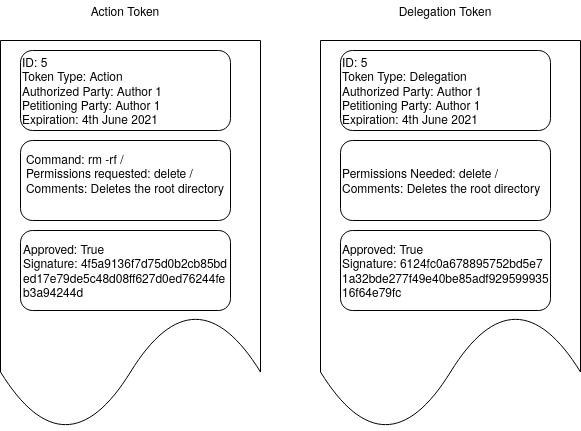
\includegraphics[width=\linewidth]{figs/TokenStructures.png}
\caption{COLBAC Token Structures}
\label{fig:Tokenformatfigure}
\end{figure}
Each token contains three sections, a header, a body, and a footer. Different
types of tokens (Action Tokens, Delegation Tokens, or Emergency Tokens) contain
different fields in their body sections. However, the headers and footers of all
token types contain the same fields. For a graphical representation of the token
format, please see Figure~\ref{fig:Tokenformatfigure}.

The first portion of a token is called the header. The header contains the
following fields:
%Header:
\begin{enumerate}
\item \textbf{Nonce/ID}:\\ 
An integer used to both identify the token and avoid replay attacks.
\item \textbf{Token Type}:\\ 
The type of token. Can only be Action, Delegation, or Emergency.
\item \textbf{Party(s) Being Authorized}:\\
A single entity or set of entities requesting authorization to perform an action
or set of actions in the Collective Sphere.
\item \textbf{Petitioning Party}:\\
The single entity petitioning for authorization. This user usually also exists
in the list of parties being authorized.
\item \textbf{Token Expiration}:\\
The expiration time of the token in Unix format.
\end{enumerate}

For Action Tokens or Emergency Tokens, the token body contains the following
fields:
\begin{enumerate}
\item \textbf{Code to be Run}:\\
The command, script, or program to be run in the Collective Sphere.
\item \textbf{Permissions Requested}:\\
A set of permissions requested to complete the task. These permissions include
negative and positive permissions, of which negative permissions take
precedence. The inclusion of both negative and positive permissions make it
easier for permissions to be specified. For example, if a folder in the
Collective Sphere contains 950 files, and the code running needs read access to
940 of them, it is easier to specify positive read permissions on the whole
folder and negative read permissions on the 10 files, rather than specify 940
positive read permissions and no negative read permissions.
\item \textbf{Comments (optional)}:\\
Comments explaining what the code included in the token does, and why it is
necessary. This field is similar to messages included in version control systems
like a Git commit message.
\end{enumerate}

For Delegation Tokens, the body contains the following fields:
\begin{enumerate}
\item \textbf{Permissions Needed}:\\
Similar to the set of permissions requested in the Action or Emergency Token
body.
\item \textbf{Comments (optional)}:\\
Similar to the comments section of the Action or Emergency Token body.
\end{enumerate}

As we can see, the Delegation Token body is similar to the Action or Emergency
Token body, except in that it does not specify the code that is running. This
design is ideal for sessions that require troubleshooting, or tasks that may
require back-and-forth between the system and the individual or group performing
the task. However, when using Delegation Tokens it is
more important to ensure that the Permissions Needed section follows the
principle of least privilege. If not, individuals can use the privileges they
gain from the Delegation Token to perform actions that were not originally
intended for their task(s). Though these actions will be logged into the
Immutable sphere, it still requires time and effort of the system users to undo
the actions of an individual who abused the power granted to them through
Delegation Tokens.

Each token, regardless of type, ends with a footer. The footer simply contains
one field, a field which states if it is approved or denied, along with a
verifiable authentication value that is difficult to predict and easy to verify,
such as an HMAC of the permission token keyed by a secret value known only to
the Reference Monitor.

\subsection{Formalizing COLBAC}
\label{sec:colbacformal}
In this section we formalize COLBAC, a collective based access control system.
To begin, we define important sets. We then go on to discuss which permissions
are possible in COLBAC, what abbreviations are used in our notation, and what
functions we rely on in our formalization. Finally, we introduce different
algorithms used by the reference monitor in our proposed model. This
formalization serves as a basis for our access control model.
\begin{definition}[Spheres of COLBAC]\label{def:spheres}
In COLBAC, a \textbf{Sphere} is a set which contains both subjects (users,
processes, etc.) and objects (files, etc.).\\
\mbox{}\\
Let $U$ be the User Sphere, $I$ be the Immutable Sphere, and $C$ be the
Collective Sphere. Let $\xi$ be the set of all subjects and objects in the
system. Let $\emptyset$ be the Empty Set. These sets have the following
properties:\\
\mbox{}\\
$U \cup I \cup C = \xi$\\
$U \cap I = \emptyset$\\
$U \cap C = \emptyset$\\
$I \cap C = \emptyset$\\
\hrule \mbox{}\\
\end{definition}

\noindent In addition to the sets above, our access control model also requires
a set of permissions, similar to the sets of permissions used in other access
control systems. These permissions will be used later when the reference monitor
is deciding whether or not to permit an action.

\begin{definition}[Permissions in COLBAC]\label{def:permissions}
$Create$ allows the creation of an object.\\
$Append$ allows a subject to append to the end of an object.\\
$Write$ allows arbitrary rights to an object. \\
$Read$ allows a subject to read from an object.\\
$Delete$ allows a subject to delete an object. \\
$Execute$ allows a subject to run an object as a program.\\
\hrule \mbox{}\\
\end{definition}

%\noindent Before introducing the main algorithms involved in COLBAC, we first
%need to define a few functions. However, to save space some shorthand is used.
%For the functions to follow, we will use the following short-hand:

\noindent The first important function we need to define is the $GetSphere$
function. When passed a subject or object, the $GetSphere$ function will return
the Sphere that the subject or object belongs to. Given the properties mentioned
in Definition~\ref{def:spheres}, we can see that a subject or object will be in
exactly one Sphere, meaning that this function will never return $NULL$ or more
than one value.

\begin{definition}[GetSphere]\label{def:getsphere}
$GetSphere(o:$ Subject or Object$) \rightarrow U$ iff $o \in U$, $C$ iff $o \in 
C$, $I$ iff $o \in I$\\
\hrule \mbox{}\\
\end{definition}

\noindent A very important building block of COLBAC is the \textbf{token}, which
is a primitive taken from Capability based access control. A token will allow a
subject which exists in $U$ to perform an action on an object that exists in
$C$. These tokens can be of type \textbf{Action}, denoted by a sub-scripted $a$,
\textbf{Delegation}, denoted by a sub-scripted $d$, or \textbf{Emergency},
denoted by a sub-scripted $e$. Before authorization, a token is first created by
a $DraftToken$ function, which calls one of the following three functions
depending on the type of token the subject wishes to create. In addition, COLBAC
requires a function to get the type of a given token.
\begin{definition}[Token Functions]\label{def:Tokens}
Let $u$ be a user of the system.\\
Let $o$ be the object or set if objects the user is attempting to access.\\
Let $p$ be the set of permissions the user is requesting.\\
Let $t$ be the type of token the user is attempting to create.\\
Let $e$ be the proposed expiration time of the token.\\
Let $c$ be the comment attached to a token, or in the case it doesn't exist,
let $c$ be $NULL$.\\
Let $a$ be the action\footnote{command, script or program} the user wants to run
in the Collective Sphere, or in the case that it doesn't exist, let $a$ be 
$NULL$.\\
Let $d$ be the set of delegates the user is proposing, or in the case where it
doesn't exist, let $d$ be $NULL$.\\
$DraftToken(u,o,p,e,a,c,t) \rightarrow T$ of type $T_{a}$ or $T_{d}$ or 
$T_{e}$\\
$DraftToken_{a}(u,o,p,e,a,c) \rightarrow T_{a} = (u,o,p,e,a,c)$\\
$DraftToken_{d}(u,o,p,e,d,c) \rightarrow T_{d} = (u,o,p,e,d,c)$\\
$DraftToken_{e}(u,o,p,a,c) \rightarrow T_{e} = (u,o,p,a,c)$\\
$GetTokenType(t:$ token$) \rightarrow \{$the type of token $t$ from $Action$,
$Delegation$, or $Emergency$\}
\hrule \mbox{}\\
\end{definition}

\noindent Unlike other capability based access control systems, COLBAC does not
rely on a centralized authority or resource owner in the system to grant
capability tokens. Instead, when a token is drafted by the user requesting it,
the token enters a $Petition$ function, which sends the token to all other
users\footnote{Here we mean human users of the system, not subjects or user
accounts on the system that don't correspond to humans.} of the system for a
participatory decision-making process on whether or not the token should be
authorized. This $Petition$ function returns a set of votes on the token $T$,
referred to as $V_{T}$, and can only be called on tokens of type \textit{action}
or \textit{delegation.}

Let's consider again the example of the democratic trade union presented in
Section~\ref{sec:introduction}. As mentioned in Section~\ref{sec:Tokentypes},
in COLBAC this change of power would occur through a Delegation Token. Relating
to the notation in Definition~\ref{def:Tokens}, if \textit{u} were a member of
the committee, $o$ was the set of files, folders, and programs needed to read,
write, and send emails, $p$ was the necessary set of permissions to perform
these actions\footnote{Such as the $Execute$ permission for the email program,
the $Create$ and $Write$ permission for temporary files, the $Read$ permission
for the files the emails are stored in, etc.}, $e$ was the expiration date of
the token\footnote{Which should be set to the last day of the mandate of the
elected body.}, $d$ was the list of all members of the committee, and $c$ was
any human-readable comment the token drafter deemed necessary. Then, the token
drafter would compute $T_{d} = DraftToken_{d}(u,o,p,e,d,c)$, and run
$Petition(T)$ as follows.

\begin{definition}[Petition Function]\label{def:petition}
Let $T$ be a token created through $DraftToken$.\\
$Petition(T) \rightarrow \{$set of votes $V_{T}$ on authorizing $T$ iff $T$ is
of type $T_{a}$ or $T_{d}$, else $NULL$\}.\\
\hrule \mbox{}\\
\end{definition}

\noindent This Petition Phase would collect votes from all of the members on the
system. The returned set of votes, $V$, can then be split into more useful
sets, such as the set of votes that affirm the authorization of $T$,
$V_{(T, Yes)}$, the set of votes that negate the authorization of $T$,
$V_{(T, No)}$, and the set of abstentions, $V_{(T, Blank)}$. After votes are
sorted into their respective sets, the process of authorizing the votes comes
down to a simple task of comparing the number of votes to fractions of voters
initially defined at system registration. Said another way, a function called
$AuthorizeToken$ will count the votes and compare the results to two security
parameters, $f$, or the fraction of yes votes required to authorize a token, and
$m$, the fraction of voters required to participate in order for a vote to be
considered. These two security parameters are chosen at the initialization of
the system, and can be changed by a successful Action Token\footnote{These
parameters cannot be changed by a delegate or by an Emergency Token. This is
discussed more in Section \ref{sec:colbacproperties}.}. If the vote is
successful, the token is then authorized by the addition of a signature field
that is difficult to predict or replicate, but easy for the reference monitor to
later verify. One example of this is a keyed HMAC.
%\begin{definition}[Sets of Votes]\label{def:votes}
%$V_{(T, Yes)} = \{v \in V$ s.t. $v = True\}$\\
%$V_{(T, No)} = \{v \in V$ s.t. $v = False\}$\\
%$V_{(T, Blank)} = \{v \in V$ s.t. $v = NULL\}$\\
%\hrule\mbox{}\\
%\end{definition}

\begin{definition}[Authorization in COLBAC]
Let $V$ be the set of all votes on token T.\\
Let $V_{(T, Yes)} = \{v \in V$ s.t. $v = True\}$\\
Let $V_{(T, No)} = \{v \in V$ s.t. $v = False\}$\\
Let $V_{(T, Blank)} = \{v \in V$ s.t. $v = NULL\}$\\
$AuthorizeToken(T,V_{T}) \rightarrow True$ iff $\frac{|V_{(T, Yes)}|}{|V|} > f
\wedge \\ \frac{|V_{(T,Yes)} \cup V_{(T, No)}|}{|V|} \ge m$, else $False$\\
\hrule\mbox{}\\
\end{definition}

The process of determining authorization in COLBAC occurs in one or two phases,
depending on which Sphere contains the object the subject wants to access.
If the object is in the User Sphere, the reference monitor simply performs a
traditional DAC check, like one would see on a typical Unix-like operating
system.

If the object is in the Collective Sphere, the subject is expected to
provide a previously authorized token or draft a new token for the reference
monitor. If the subject provides a previously authorized token, the validity of
that token is checked, and if it is valid, the action is taken. If the subject
does not have a valid token, they instead provide a draft token. The reference
monitor then takes this draft token and enters the Petition Phase, where all
users of the system are given the opportunity to vote on the token. If the
petition succeeds, the token is authorized and returned to the subject. If the
petition fails, the token is not returned. In either case, the submission of the
token to the reference monitor is logged in the Immutable Sphere. In the example
provided in Section~\ref{sec:introduction}, all of the data required to access
the collective email exists in the Collective Sphere.

If the object the subject is trying to access is in the Immutable Sphere, the
reference monitor performs a very simple access control check. If the type of
access on the resource in the Immutable Sphere is a $read$ operation, it always
succeeds. This is to provide transparency on the different operations that are
attempted in the Collective Sphere, since the Immutable Sphere mainly contains
logs of what was done in the Collective Sphere. If the type of access on the
resource in the Immutable Sphere is a $write$ operation, it always fails, since
$write$ operations can arbitrarily write to any portion of a file. Likewise,
$delete$ operations and $execute$ operations always fail. If the operation is a
$create$ or $append$ operation, the reference monitor must check that the
subject has a valid token to do so. If not, they may not perform the action.
The reference monitor, however, may always append or create in the Immutable
Sphere.

An algorithmic representation of these access control decisions are included in
Algorithm~\ref{alg:main}. To continue with our example from Section
\ref{sec:introduction}, imagine that a member of the committee wants to read an
email in the Collective Sphere. We can see that $GetSphere(o)$ would return $C$,
since the email program exists in the Collective Sphere. Thus, the block of code
from lines 14 to 20 would be executed, and the token would be checked. Assuming
that the previous vote on the Petition Phase for the Delegation Token has
passed, line 14 would return the non-NULL Delegation Token that $u$ has as a
member of the elected committee. Then, since the action that they wish to
perform (read an email) is covered by the permissions of the Delegation Token
$T$, the action will be logged on line 17 and then performed on line 18.
However, if $u$ were not a member of the committee, then the $GetToken$ function
would return NULL, or would return tokens that do not have the relevant
permissions. As such, lines 22 -- 32 or line 19 would be executed, respectively.

\begin{algorithm}
\caption{The main decision making process of COLBAC}
\label{alg:main}
\begin{algorithmic}[1]
\State Let $u$ be a user of the system.
\State Let $s$ be the subject attempting access.
\State Let $o$ be the object or set if objects the user is attempting to access.
\State Let $p$ be the set of permissions the user is requesting.
\State Let $t$ be the type of token the user is attempting to create.
\State Let $e$ be the proposed expiration time of the token.
\State Let $c$ be the comment attached to a token, or in the case it doesn't exist,
let $c$ be $NULL$.
\State Let $a$ be the action the user wants to run in the Collective Sphere, or in the
case that it doesn't exist, let $a$ be $NULL$.
\State Let $d$ be the set of delegates the user is proposing, or in the case where it
doesn't exist, let $d$ be $NULL$.
\State Let $DAC(s :$ Subject$, o:$ Object$)$ be a Discretionary Access Control
system.
\If{$GetSphere(o)=U$}
    \State Return $DAC(s,o)$
\ElsIf{$GetSphere(o)=C$}
    \State $T = GetToken(u)$
    \If{$T \ne NULL$}
        \If{IsValid($C, T, a$)}
            \State LogAction($a, u$)
            \State PerformAction($a$)
        \Else
            \State LogFailedAction($a, u$)
        \EndIf
    \Else
        \State $T = DraftToken(u,o,p,t,e,c,a,d)$
        \If{$GetTokenType(T) \in (T_{a}, T_{d})$}
            \State $V_{T} = Petition(T)$
            \State $V_{(T, Yes)} = \{v \in V$ s.t. $v = True\}.$
            \State $V_{(T, No)} = \{v \in V$ s.t. $v = False\}.$
            \State $V_{(T, Blank)} = \{v \in V$ s.t. $v = NULL\}$.
            \If{$AuthorizeToken(T, V_{(T, Yes)}, V_{(T, No)}, V_{(T, Blank)},f, m)$}
                \State LogSuccess($T$)
                \State Return $T$
            \Else
                \State LogFailure($T$)
            \EndIf
        \EndIf
    \EndIf
\Else
    \State $T = GetToken(u)$
    \If{IsValid($I, T, a$)}
        \State LogAction($a, u$)
        \State PerformAction($a$)
    \Else
        \State LogFailedAction($a, u$)
    \EndIf
\EndIf
\end{algorithmic}
\end{algorithm}

Perhaps the most important part of this logic lies in the IsValid function. This
function must ensure that the token itself has been issued by the reference
monitor, that the token has not expired, and that the permissions of the actions
that the token grants are consistent with what the action is attempting to do.
In the case that one of these three conditions is not true, the reference
monitor must not perform an action. We present the logic of the IsValid function
in Algorithm~\ref{alg:isvalid}.

To understand this Algorithm we still need to introduce one more function
definition. In order to be able to decide whether or not a given action should
be allowed, the reference monitor must be able to see what permissions the
action the subject is supplying requires. Thus, we introduce the
GetRequiredPermissions function as follows. This function works on the level of
commands, instead of actions, to allow for granular identification of which
portion of the action is causing issues (if indeed the action is longer than one
command).

\begin{definition}
GetRequiredPermissions$(c:$ Command$) \rightarrow$ \{the set of permissions,
$p'$ needed to complete the proposed command.\}\\
PermissionType$(p:$ Permission$) \rightarrow $ \{the type of access the
permission is requesting among the permissions listed in Definition
\ref{def:permissions}\}\\
\hrule\mbox{}\\
\end{definition}

\begin{algorithm}
\caption{The IsValid function of COLBAC.}
\label{alg:isvalid}
\begin{algorithmic}[1]
\Procedure{IsValid}{$S$: Sphere, $T$: Token, $a$: Action}
\State Let $C$ be the Collective Sphere.
\State Let $I$ be the Immutable Sphere.
\If{$S = C$}
    \If{$GetTokenType(T) \neq T_{e}$}
        \For{$c \in a$} \Comment{For each command in the action}
            \State $p =$ GetRequiredPermissions$(c)$
            \If{$p \notin T.p$}
                \State Return $False$
            \EndIf
        \EndFor
        \State Return $True$
    \Else
        \State $p =$ GetRequiredPermissions$(c)$
        \If{CheckEmergencyPermissions($p$) $\neq True$}
            \State Return $False$
        \EndIf
        \State Return $True$
    \EndIf
\ElsIf{$S = I$}
    \For{$c \in a$} \Comment{For each command in the action}
        \State $p$ = GetRequiredPermissions$(c)$
        \If{PermissionType($p$) $\in (write, delete, execute)$}
            \State Return $False$
        \ElsIf{PermissionType($p$) $\in (create, append)$}
            \If{$p \notin T.p$}
                \State Return $False$
            \EndIf
            \State Return $True$
        \Else \Comment{The permission is read}
            \State Return $True$
        \EndIf
    \EndFor
\EndIf
\EndProcedure
\end{algorithmic}
\end{algorithm}

In this paper we leave CheckEmergencyPermissions as yet undefined, but discuss
some possibilities for this function in Section~\ref{sec:colbacproperties}.

\subsection{Properties of COLBAC}
\label{sec:colbacproperties}
In Section~\ref{sec:colbacdesign} we introduced the design of COLBAC, an access
control system meant to serve as a primitive that can be used to achieve a more
horizontal form of security. In Section~\ref{sec:colbacformal} we presented a
more formal definition of the system, filling in some of the details of how the
system worked.

As stated in Section~\ref{sec:colbacrequirements}, the goals of the system
design were to provide flexible and dynamic horizontality, and to provide
transparency such that individuals participating in the system could reasonably
participate in the decision-making process. Through the design of COLBAC we have
created an access control system that meets these goals. We achieve flexible and
dynamic horizontality in our design through the modification of our two security
parameters, $f$ and $m$. We achieve transparency through the use of the
Immutable Sphere, and the logging that our reference monitor does during its
operation (as described in Algorithm~\ref{alg:main}.

Though our design does provide for flexible and dynamic horizontality, it does
not allow for every level of horizontality. For example, in our design a
strictly-hierarchical approach is not possible: even if $f$ is set to
$\frac{1}{n}$, where $n$ is the number of users, that simply means that one
person needs to vote in favor to authorize an action, but it does not say
\textit{which} individual has that power, meaning that any single vote from any
user is capable of authorizing an action. This is far from a dictatorial
structure, in which all power is fixed in the hands of one individual or a small set of
individuals.

This design does allow for many different expressions of horizontal structures,
however. For example, because of the existence of Delegation Tokens which expire,
our design allows for an authorization structure that reflects those of
representative democracies, where elected individuals preside over certain
responsibilities in the system. However, if the collective does not approve of
how the elected individual is performing their duties, our solution allows for
users to call for a democratic vote that invalidates the token of the delegate,
thus forcing a new delegate to be chosen, or bringing the responsibility back
into the collective.

More, our system allows for Action Tokens to modify the values of $f$ and $m$,
thus making it possible for an organization to adjust how many individuals in
the collective must agree on authorizing a token in order for the token to be
authorized. This allows the organization to decide if they want to work with
a full consensus based approach, a super majority approach, a majority approach,
or something else entirely. A consequence of this system is that it is easier to
require \textbf{more} consensus than it is to require \textbf{less} consensus.
This property is obvious when one realizes that if an organization calls a vote
to switch from $f$ to $f'$ where $f > f'$, that action token still needs $f$
votes, the larger number, to become authorized. However, if the organization
wants to require \textbf{more} consensus, in other words a user petitions a
token to change from $f$ to $f'$ where $f < f'$, then that vote requires $f$
votes, the smaller number of the two, to be authorized. A similar claim can be
made about the amount of interaction required, which would be affected by
changing the security parameter $m$.

Another interesting property of this system is that it contains in it the
inalienable right to vote. Whenever a vote is called, the reference monitor does
not send it to a small set of individuals who are marked as having a right to
vote. Instead, it sends it to all individuals who are a part of the system.
Thus, in the COLBAC system the right to vote is inalienable as long as one
remains part of the system. Likewise, because the reference monitor grants all
read access to any object in the Immutable Sphere and disallows any deletions or
arbitrary writes in the Immutable Sphere, transparency of the system is
guaranteed so long as the reference monitor behaves according to the system
design.

However, in order to avoid the equivalent of a coup d'\'etat on the system, we
must set some limitations of what certain tokens can do. For example, if an 
individual user of the system wishes to perform a coup d'\'etat, one approach
would be to use an emergency token to set $f$ and $m$ to $\frac{1}{n}$ where $n$
is the number of users in the system, then create and authorize action tokens to
remove users from the system until only user accounts that are loyal to that
user remain. To avoid this, there must be limitations on what Emergency Tokens
and delegation tokens can do. For this case specifically, emergency and
Delegation Tokens must not be able to alter the values of $f$ and $m$. Similarly
there must be a limitation on the number of emergency tokens an individual has,
and individuals with access to delegation tokens must not be able to remove many
members. It is likely that even more restrictions are required to maintain the
safety of the system, but we leave the identification of those limitations, and
further analysis of the properties of COLBAC, to future work.

%\subsection{Limitations of COLBAC}
%\label{sec:colbaclimitations}
%Like all systems, COLBAC is not perfect, and suffers from limitations. Perhaps
%one of the most obvious limitations of COLBAC is its usability and user
%experience. Creating a horizontal access control system with democratic
%participation requires the system to interact with its users much more than a
%traditional operating system. Users will be expected to vote on many Tokens in
%the Petition Phase, and this may cause fatigue in some users. Additionally, 
%having horizontal technological solutions relies on the digital literacy of the
%users: users who know how to audit the commands sent in the petition phase have
%a deeper understanding of the potential effects of their vote. However, these
%problems may be solved through interface design, and through iterative
%development of the access control system.
%
%Additionally, COLBAC has a limitation regarding \textit{which} democratic governance structures
%it can represent. For example, a purely elected representative structure without
%referendums is impossible to create using COLBAC, since the right to petition
%a Token is inalienable in COLBAC. While this may be seen as a positive for many
%horizontally-run organizations, some may also view it as a negative. Finally,
%currently COLBAC does not allow for different values of $f$ and $m$ per file.
%Future research may be needed to determine how this would affect the properties
%of COLBAC, and if it may introduce new attacks.
%
%More, COLBAC focuses only on voting, with strictly set options of yes, no, and
%abstention. Future work should look into more forms of democratic participation,
%including but not limited to random sampling, run-off voting (instant, and
%round based), and more. Another potentially useful feature could be the concept
%of an amendment, or an ability to introduce a change to a petition such as
%removing a permission, or fixing a line of code in the action.


% Access Control:
% La-Padula, Biba, strictly hierarchical
% DAC based on individualistic regulation of files, overwritable by admin on
%    most systems.
% MAC or RBAC seem to be desirable for horizontal security, but how do we update
%    policies?

% Bitcoin:
% attempt at horizontal, democratic control of currency.
% Regulatable with 51%.
% suffers from centralization as it goes on due to its competative nature.

%\begin{enumerate}
%\item Case study: Code review.
%\item Case study: Peer review.
%\end{enumerate}

%Conclusion: Security is purely horizontal when the policies and enforcement are
%handled via direct democratic vote. Horizontality is a spectrum, ranging from
%hierarchical (one person with decision making power) to purely horizontal.
%Examples of spots on the spectrum include:
%\begin{itemize}
%\item direct democracy / consensus cooperatives
%\item Random review (i.e. code review)
%\item random/elected representatives w/ early revocation
%\item random/elected representatives w/o early revocation
%\item appointed representatives
%\item hierarchical
%\end{itemize}

%Very few spots on this spectrum are represented in current techniques and
%techologies. Mostly the hierarchical approach is developed because of its
%continued use in business and government. As that changes, cybesecurity needs to
%be ahead of the curve and create technologies for the organizations and
%businesses that sit on the other portions of this spectrum.


\section{COLBAC: Collective Based Access Control}
\label{sec:colbac}
As discussed in previous sections, the choice of certain software, protocols, or
techniques such as X509 certificates or PGP web of trust has implications in the
level of horizontality possible for systems built on top of those software,
protocols, or techniques. How, then, can we build a foundation such that
organizations of different horizontality can use the same foundation and arrive
at much differently structured organizations?

In this section we describe Collective Based Access Control, or COLBAC: our
approach to a dynamic horizontality access control system. We begin by
describing its requirements, focusing on the dynamic horizontality that
separates COLBAC from other access control systems. We then define the system
itself. Finally, we discuss the properties and in Section~\ref{sec:limitations}
we discuss the limitations of this system. Though this is, to our knowledge, the
first attempt at defining a collective based access control system with dynamic
and flexible horizontality, it is far from the only potential approach. Section
\ref{sec:future_work} discusses some potential future work to improve upon it.

To our knowledge COLBAC is the first attempt to incorporate democratic processes
into access control. However, democracy is a complex concept, and COLBAC only
incorporates some aspects of democracy. For example, solution is not utilized
at all in COLBAC. For our definition of the \textit{Demos}, we consider all
members of a system using COLBAC do be part of the \textit{Demos} and thus
eligible to vote. Our design of COLBAC also assumes there exists an external
channel for deliberation that is used by all members of the \textit{Demos}, and
that there may exist external channels for other forms of decision-making.
However, every decision made in these external channels that affects the system
must eventually become a vote within COLBAC.

Given these assumptions and the design of COLBAC, we can see that COLBAC allows
for a large variety of different democratic governance schemes. More direct
forms of democracy can be done using Action Tokens, and elective representation
can be done using Delegation Tokens\footnote{These types of tokens are described
in Section~\ref{sec:Tokentypes}}. The spectrum between full consensus and
majority decision-making is represented through the security parameter $f$ and
the decision of how much participation is required per vote and, therefore, how
difficult it is to create a quorum can be fine-tuned using the security
parameter $m$\footnote{These security parameters are described in Section
\ref{sec:colbacdesign}}.

\subsection{System Requirements}
\label{sec:colbacrequirements}
COLBAC is aimed at addressing a novel requirement in Cybersecurity research:
access control and authorization given an organization with dynamic levels of
horizontal control. Though previous approaches exist for hierarchical access
control (such as MAC, RBAC, etc.), to our knowledge no access control model
exists for organizations of dynamic and flexible horizontality. To realize
this, our solution must be able to be flexible in terms of horizontality. Said
another way, our system must not assume or define a pre-determined threshold for
horizontal control, i.e., it must not assume majority, or super-majority, or
full consensus is the preferred method of democratic participation. Instead,
the threshold must be configured by the collective itself, and must be able to
be changed when necessary. This allows for rapid temporary centralization of the
system to respond to crises, or to perform a task that requires expertise that
few members of the collective contain. However, these moments of centralization
must be quick to expire and easy to override in order to prevent abuse of
centralized power. Said another way, it must always be easier for the collective
to return to more horizontal control than for a centralized entity to maintain
control over the system.

However, it makes no sense to have horizontal or democratic control without
transparency. An individual cannot meaningfully vote or otherwise decide on a
practice, or place confidence in a representative, without understanding what
the action is going to take place, and what actions have been taken in the past.
More, if authority is abused, the collective must be able to notice the abuse,
and remove the powers that allowed the abuse to take place. Thus, we can see
that any horizontal access control system requires transparency. Towards this
end, our system must have a method of logging information about the actions of
individuals and the collective that is immutable and available.

\subsection{System Design}
\label{sec:colbacdesign}
COLBAC presents a solution to access control that relies on the collective.
However, as will be discussed later in this section, not all objects on the
system will need to be collectively controlled or administered. As such, we
define three distinct \textit{spheres} of the system, or areas that require
different approaches to access control. These spheres are the \textbf{Collective
Sphere}, the \textbf{User Spheres}, and the \textbf{Immutable Sphere}.

In order to achieve different degrees of horizontality, there must be a portion
of the system that is controlled not by any individual user of the system, but
by some democratic process of the users of the system. We call this portion of
the system the \textbf{Collective Sphere}, as it contains programs, files, and
other resources only accessed based on collective authorization. In any
horizontal system, the administrative functions of the operating system would
need to exist within this portion of the system to allow for true collective
control. Additionally, all services that the collective offers, or official
sources of collective information, must also exist in this sphere.

However, not everything should be directly managed by the collective. Individual
users may have their own files and programs, which they intend to use only in
ways that do not affect other users of the system or the resources of the
collective\footnote{We can think of these as the home directories of users in
modern Unix-like systems.}. This sphere, called the \textbf{User Sphere},
can use traditional DAC systems like modern Unix-like systems without affecting
the horizontality of the system as a whole.

Finally, to have meaningful control of the system we must have transparency. To
achieve this, a system must have an \textbf{Immutable Sphere}, or a portion of
the file system and programs that cannot be altered once written to, including
by democratic control. This allows for the system to provide append-only logs
that are vital to maintaining collective control, as described later in this
section. Additionally, this section can hold a list of inalienable rights that
each participant in the system has, such as the right to a vote.

When the system is first installed, a \textit{Registration Phase} will occur.
During this phase, at least 3 users will be signed up in the system. These users
will need to supply their public keys, which correspond to offline private keys,
since they will be needed for later interactions with the system. In addition to
supplying their public keys, the users will need to decide on an initial
fraction $f$ and a minimum fraction $m$ that will be used for action and
delegation petitions, as explained later.

After the system is set up, users can interact with objects in the User Sphere
as they would in any other system. However, to interact with any objects in the
Collective Sphere, users would need to follow a specific authorization
procedure consisting of three phases: the \textit{Draft Phase}, the 
\textit{Petition Phase}, and the \textit{Authorization Phase}.

In the Draft Phase, depending on the action the user wishes to perform, they
will write the code or commands that will interact with objects in the
Collective Sphere, or will identify the permissions they will need to accomplish
their task or tasks. At the end of this process, the user will have a draft
Action or Delegation Token, as described later in Sections \ref{sec:Tokentypes}
and \ref{sec:Tokenformat}.

After the user has completed their token, they move on to the Petition Phase. In
this phase the user sends their draft token to the reference monitor running on
the system. This reference monitor will then forward the draft token to all
other members of the system and ask for a vote. The users will then vote one of
the following ways: yes, no, or abstain\footnote{It is important to mention that
this is not the only way of performing democratic participation. However, other
models of democratic participation are left to future work.}. The system will
wait for a pre-configured amount of time before marking all individuals who did not
vote as abstaining.

After all votes are collected or the response period has timed out, the system
enters the authorization phase. During the action phase the reference monitor
counts all of the votes. If the number of votes divided by the total number of
users is greater than or equal to $m$, and the fraction of yes votes to the
total number of votes is greater than or equal to $f$, the petition is
considered successful and the token is returned to the petitioning user. In
addition to taking the action, the system logs the action in log files held in
the immutable sphere. However, if the number of all votes divided by the total
number of users is less than $m$ or if the number of yes votes divided by the
total number of votes is less than $f$, the petition fails, and the attempted
action is logged in the immutable sphere.

\subsection{Types of Tokens}
\label{sec:Tokentypes}
As the previous section demonstrates, the token is the main form of interacting
with the Collective Sphere. Users who wish to affect the Collective Sphere do
so by creating a token which is then voted on by the users of the system. In
order to facilitate easy interaction with the COLBAC system, there are multiple
types of tokens.

The first token is called the \textbf{Action Token}. This token allows a single
command, a small script, or a program to be run in the Collective Sphere, and to
enjoy Collective Sphere access. This is the most straightforward type of token,
since everything the token will allow to occur is known during the Petition
Phase. However, this type of token is rigid and inflexible. If there is an error
in the command, or in the code, a user would need to re-enter the Draft Phase,
fix the error, and re-enter the Petition Phase to authorize a new token. The
more a single Action Token attempts to do, the more likely there will be errors,
causing frustration for both the users drafting the tokens and the users voting
on them.

To avoid these issues, COLBAC also allows for \textbf{Delegation Tokens}, which
allow the drafting user to act in the Collective Sphere for a given set of time,
and with a given set of restrictions. The procedure is obtaining a Delegation
Token is the same as that for an Action Token. However, the information that
would be put in the token would be slightly different. The format for Action
Tokens and Delegation Tokens are shown in Section~\ref{sec:Tokenformat}.

Consider the example of the democratically run trade union introduced in Section 
\ref{sec:introduction}. In this example, a new communication committee was put
in power though a slate of democratic elections. However, former individuals who
had access to read the emails that arrived to the collective's inbox did not
allow members of the new committee to read or send emails. If this trade union
had been using COLBAC, after the elections a Delegation Token would have been
drafted to grant the new committee access to both read and send emails. This
Delegation Token would then gone through a Petition Phase, where presumably it
would pass\footnote{This assumption is based off of the results of the
democratic elections that occurred before.}. Thus, the individuals previously in
charge of email would be incapable of denying access to the new committee.

There are some instances in which one needs to respond to emergency situations
as soon as possible, and cannot wait for a slow authorization process by a
potentially large set of users. To accommodate these situations, COLBAC has an
\textbf{Emergency Token}. These tokens allow users to run short scripts, single
commands, or small programs in the Collective Sphere without immediate
authorization. However, this action is immediately logged and all users are
informed by the Reference Monitor that an Emergency Token was used. In the case
that an Emergency Token was incorrectly used (say, to overwrite the result of
a democratically made decision), a member can create a new Action Token to
undo the actions of the Emergency Token, which will be pushed to a Petition
Phase for democratic decision making. To avoid large-scale misuse of the
Emergency Token, and to avoid Emergency Token Wars\footnote{We define Emergency
Token Wars as instances in which different members in the organization use
Emergency Tokens to undo the actions taken in the name of the collective.},
each member only has a small number of Emergency Tokens for a given period of
time. Additionally, there are limits placed on what can be done with Emergency
Tokens.

\subsection{Token Format}
\label{sec:Tokenformat}
\begin{figure}
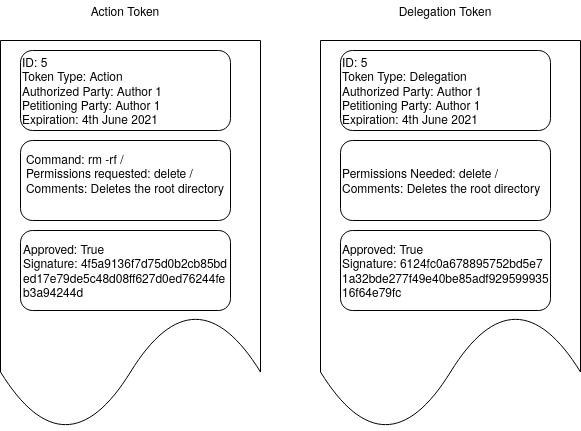
\includegraphics[width=\linewidth]{figs/TokenStructures.png}
\caption{COLBAC Token Structures}
\label{fig:Tokenformatfigure}
\end{figure}
Each token contains three sections, a header, a body, and a footer. Different
types of tokens (Action Tokens, Delegation Tokens, or Emergency Tokens) contain
different fields in their body sections. However, the headers and footers of all
token types contain the same fields. For a graphical representation of the token
format, please see Figure~\ref{fig:Tokenformatfigure}.

The first portion of a token is called the header. The header contains the
following fields:
%Header:
\begin{enumerate}
\item \textbf{Nonce/ID}:\\ 
An integer used to both identify the token and avoid replay attacks.
\item \textbf{Token Type}:\\ 
The type of token. Can only be Action, Delegation, or Emergency.
\item \textbf{Party(s) Being Authorized}:\\
A single entity or set of entities requesting authorization to perform an action
or set of actions in the Collective Sphere.
\item \textbf{Petitioning Party}:\\
The single entity petitioning for authorization. This user usually also exists
in the list of parties being authorized.
\item \textbf{Token Expiration}:\\
The expiration time of the token in Unix format.
\end{enumerate}

For Action Tokens or Emergency Tokens, the token body contains the following
fields:
\begin{enumerate}
\item \textbf{Code to be Run}:\\
The command, script, or program to be run in the Collective Sphere.
\item \textbf{Permissions Requested}:\\
A set of permissions requested to complete the task. These permissions include
negative and positive permissions, of which negative permissions take
precedence. The inclusion of both negative and positive permissions make it
easier for permissions to be specified. For example, if a folder in the
Collective Sphere contains 950 files, and the code running needs read access to
940 of them, it is easier to specify positive read permissions on the whole
folder and negative read permissions on the 10 files, rather than specify 940
positive read permissions and no negative read permissions.
\item \textbf{Comments (optional)}:\\
Comments explaining what the code included in the token does, and why it is
necessary. This field is similar to messages included in version control systems
like a Git commit message.
\end{enumerate}

For Delegation Tokens, the body contains the following fields:
\begin{enumerate}
\item \textbf{Permissions Needed}:\\
Similar to the set of permissions requested in the Action or Emergency Token
body.
\item \textbf{Comments (optional)}:\\
Similar to the comments section of the Action or Emergency Token body.
\end{enumerate}

As we can see, the Delegation Token body is similar to the Action or Emergency
Token body, except in that it does not specify the code that is running. This
design is ideal for sessions that require troubleshooting, or tasks that may
require back-and-forth between the system and the individual or group performing
the task. However, when using Delegation Tokens it is
more important to ensure that the Permissions Needed section follows the
principle of least privilege. If not, individuals can use the privileges they
gain from the Delegation Token to perform actions that were not originally
intended for their task(s). Though these actions will be logged into the
Immutable sphere, it still requires time and effort of the system users to undo
the actions of an individual who abused the power granted to them through
Delegation Tokens.

Each token, regardless of type, ends with a footer. The footer simply contains
one field, a field which states if it is approved or denied, along with a
verifiable authentication value that is difficult to predict and easy to verify,
such as an HMAC of the permission token keyed by a secret value known only to
the Reference Monitor.

\subsection{Formalizing COLBAC}
\label{sec:colbacformal}
In this section we formalize COLBAC, a collective based access control system.
To begin, we define important sets. We then go on to discuss which permissions
are possible in COLBAC, what abbreviations are used in our notation, and what
functions we rely on in our formalization. Finally, we introduce different
algorithms used by the reference monitor in our proposed model. This
formalization serves as a basis for our access control model.
\begin{definition}[Spheres of COLBAC]\label{def:spheres}
In COLBAC, a \textbf{Sphere} is a set which contains both subjects (users,
processes, etc.) and objects (files, etc.).\\
\mbox{}\\
Let $U$ be the User Sphere, $I$ be the Immutable Sphere, and $C$ be the
Collective Sphere. Let $\xi$ be the set of all subjects and objects in the
system. Let $\emptyset$ be the Empty Set. These sets have the following
properties:\\
\mbox{}\\
$U \cup I \cup C = \xi$\\
$U \cap I = \emptyset$\\
$U \cap C = \emptyset$\\
$I \cap C = \emptyset$\\
\hrule \mbox{}\\
\end{definition}

\noindent In addition to the sets above, our access control model also requires
a set of permissions, similar to the sets of permissions used in other access
control systems. These permissions will be used later when the reference monitor
is deciding whether or not to permit an action.

\begin{definition}[Permissions in COLBAC]\label{def:permissions}
$Create$ allows the creation of an object.\\
$Append$ allows a subject to append to the end of an object.\\
$Write$ allows arbitrary rights to an object. \\
$Read$ allows a subject to read from an object.\\
$Delete$ allows a subject to delete an object. \\
$Execute$ allows a subject to run an object as a program.\\
\hrule \mbox{}\\
\end{definition}

%\noindent Before introducing the main algorithms involved in COLBAC, we first
%need to define a few functions. However, to save space some shorthand is used.
%For the functions to follow, we will use the following short-hand:

\noindent The first important function we need to define is the $GetSphere$
function. When passed a subject or object, the $GetSphere$ function will return
the Sphere that the subject or object belongs to. Given the properties mentioned
in Definition~\ref{def:spheres}, we can see that a subject or object will be in
exactly one Sphere, meaning that this function will never return $NULL$ or more
than one value.

\begin{definition}[GetSphere]\label{def:getsphere}
$GetSphere(o:$ Subject or Object$) \rightarrow U$ iff $o \in U$, $C$ iff $o \in 
C$, $I$ iff $o \in I$\\
\hrule \mbox{}\\
\end{definition}

\noindent A very important building block of COLBAC is the \textbf{token}, which
is a primitive taken from Capability based access control. A token will allow a
subject which exists in $U$ to perform an action on an object that exists in
$C$. These tokens can be of type \textbf{Action}, denoted by a sub-scripted $a$,
\textbf{Delegation}, denoted by a sub-scripted $d$, or \textbf{Emergency},
denoted by a sub-scripted $e$. Before authorization, a token is first created by
a $DraftToken$ function, which calls one of the following three functions
depending on the type of token the subject wishes to create. In addition, COLBAC
requires a function to get the type of a given token.
\begin{definition}[Token Functions]\label{def:Tokens}
Let $u$ be a user of the system.\\
Let $o$ be the object or set if objects the user is attempting to access.\\
Let $p$ be the set of permissions the user is requesting.\\
Let $t$ be the type of token the user is attempting to create.\\
Let $e$ be the proposed expiration time of the token.\\
Let $c$ be the comment attached to a token, or in the case it doesn't exist,
let $c$ be $NULL$.\\
Let $a$ be the action\footnote{command, script or program} the user wants to run
in the Collective Sphere, or in the case that it doesn't exist, let $a$ be 
$NULL$.\\
Let $d$ be the set of delegates the user is proposing, or in the case where it
doesn't exist, let $d$ be $NULL$.\\
$DraftToken(u,o,p,e,a,c,t) \rightarrow T$ of type $T_{a}$ or $T_{d}$ or 
$T_{e}$\\
$DraftToken_{a}(u,o,p,e,a,c) \rightarrow T_{a} = (u,o,p,e,a,c)$\\
$DraftToken_{d}(u,o,p,e,d,c) \rightarrow T_{d} = (u,o,p,e,d,c)$\\
$DraftToken_{e}(u,o,p,a,c) \rightarrow T_{e} = (u,o,p,a,c)$\\
$GetTokenType(t:$ token$) \rightarrow \{$the type of token $t$ from $Action$,
$Delegation$, or $Emergency$\}
\hrule \mbox{}\\
\end{definition}

\noindent Unlike other capability based access control systems, COLBAC does not
rely on a centralized authority or resource owner in the system to grant
capability tokens. Instead, when a token is drafted by the user requesting it,
the token enters a $Petition$ function, which sends the token to all other
users\footnote{Here we mean human users of the system, not subjects or user
accounts on the system that don't correspond to humans.} of the system for a
participatory decision-making process on whether or not the token should be
authorized. This $Petition$ function returns a set of votes on the token $T$,
referred to as $V_{T}$, and can only be called on tokens of type \textit{action}
or \textit{delegation.}

Let's consider again the example of the democratic trade union presented in
Section~\ref{sec:introduction}. As mentioned in Section~\ref{sec:Tokentypes},
in COLBAC this change of power would occur through a Delegation Token. Relating
to the notation in Definition~\ref{def:Tokens}, if \textit{u} were a member of
the committee, $o$ was the set of files, folders, and programs needed to read,
write, and send emails, $p$ was the necessary set of permissions to perform
these actions\footnote{Such as the $Execute$ permission for the email program,
the $Create$ and $Write$ permission for temporary files, the $Read$ permission
for the files the emails are stored in, etc.}, $e$ was the expiration date of
the token\footnote{Which should be set to the last day of the mandate of the
elected body.}, $d$ was the list of all members of the committee, and $c$ was
any human-readable comment the token drafter deemed necessary. Then, the token
drafter would compute $T_{d} = DraftToken_{d}(u,o,p,e,d,c)$, and run
$Petition(T)$ as follows.

\begin{definition}[Petition Function]\label{def:petition}
Let $T$ be a token created through $DraftToken$.\\
$Petition(T) \rightarrow \{$set of votes $V_{T}$ on authorizing $T$ iff $T$ is
of type $T_{a}$ or $T_{d}$, else $NULL$\}.\\
\hrule \mbox{}\\
\end{definition}

\noindent This Petition Phase would collect votes from all of the members on the
system. The returned set of votes, $V$, can then be split into more useful
sets, such as the set of votes that affirm the authorization of $T$,
$V_{(T, Yes)}$, the set of votes that negate the authorization of $T$,
$V_{(T, No)}$, and the set of abstentions, $V_{(T, Blank)}$. After votes are
sorted into their respective sets, the process of authorizing the votes comes
down to a simple task of comparing the number of votes to fractions of voters
initially defined at system registration. Said another way, a function called
$AuthorizeToken$ will count the votes and compare the results to two security
parameters, $f$, or the fraction of yes votes required to authorize a token, and
$m$, the fraction of voters required to participate in order for a vote to be
considered. These two security parameters are chosen at the initialization of
the system, and can be changed by a successful Action Token\footnote{These
parameters cannot be changed by a delegate or by an Emergency Token. This is
discussed more in Section \ref{sec:colbacproperties}.}. If the vote is
successful, the token is then authorized by the addition of a signature field
that is difficult to predict or replicate, but easy for the reference monitor to
later verify. One example of this is a keyed HMAC.
%\begin{definition}[Sets of Votes]\label{def:votes}
%$V_{(T, Yes)} = \{v \in V$ s.t. $v = True\}$\\
%$V_{(T, No)} = \{v \in V$ s.t. $v = False\}$\\
%$V_{(T, Blank)} = \{v \in V$ s.t. $v = NULL\}$\\
%\hrule\mbox{}\\
%\end{definition}

\begin{definition}[Authorization in COLBAC]
Let $V$ be the set of all votes on token T.\\
Let $V_{(T, Yes)} = \{v \in V$ s.t. $v = True\}$\\
Let $V_{(T, No)} = \{v \in V$ s.t. $v = False\}$\\
Let $V_{(T, Blank)} = \{v \in V$ s.t. $v = NULL\}$\\
$AuthorizeToken(T,V_{T}) \rightarrow True$ iff $\frac{|V_{(T, Yes)}|}{|V|} > f
\wedge \\ \frac{|V_{(T,Yes)} \cup V_{(T, No)}|}{|V|} \ge m$, else $False$\\
\hrule\mbox{}\\
\end{definition}

The process of determining authorization in COLBAC occurs in one or two phases,
depending on which Sphere contains the object the subject wants to access.
If the object is in the User Sphere, the reference monitor simply performs a
traditional DAC check, like one would see on a typical Unix-like operating
system.

If the object is in the Collective Sphere, the subject is expected to
provide a previously authorized token or draft a new token for the reference
monitor. If the subject provides a previously authorized token, the validity of
that token is checked, and if it is valid, the action is taken. If the subject
does not have a valid token, they instead provide a draft token. The reference
monitor then takes this draft token and enters the Petition Phase, where all
users of the system are given the opportunity to vote on the token. If the
petition succeeds, the token is authorized and returned to the subject. If the
petition fails, the token is not returned. In either case, the submission of the
token to the reference monitor is logged in the Immutable Sphere. In the example
provided in Section~\ref{sec:introduction}, all of the data required to access
the collective email exists in the Collective Sphere.

If the object the subject is trying to access is in the Immutable Sphere, the
reference monitor performs a very simple access control check. If the type of
access on the resource in the Immutable Sphere is a $read$ operation, it always
succeeds. This is to provide transparency on the different operations that are
attempted in the Collective Sphere, since the Immutable Sphere mainly contains
logs of what was done in the Collective Sphere. If the type of access on the
resource in the Immutable Sphere is a $write$ operation, it always fails, since
$write$ operations can arbitrarily write to any portion of a file. Likewise,
$delete$ operations and $execute$ operations always fail. If the operation is a
$create$ or $append$ operation, the reference monitor must check that the
subject has a valid token to do so. If not, they may not perform the action.
The reference monitor, however, may always append or create in the Immutable
Sphere.

An algorithmic representation of these access control decisions are included in
Algorithm~\ref{alg:main}. To continue with our example from Section
\ref{sec:introduction}, imagine that a member of the committee wants to read an
email in the Collective Sphere. We can see that $GetSphere(o)$ would return $C$,
since the email program exists in the Collective Sphere. Thus, the block of code
from lines 14 to 20 would be executed, and the token would be checked. Assuming
that the previous vote on the Petition Phase for the Delegation Token has
passed, line 14 would return the non-NULL Delegation Token that $u$ has as a
member of the elected committee. Then, since the action that they wish to
perform (read an email) is covered by the permissions of the Delegation Token
$T$, the action will be logged on line 17 and then performed on line 18.
However, if $u$ were not a member of the committee, then the $GetToken$ function
would return NULL, or would return tokens that do not have the relevant
permissions. As such, lines 22 -- 32 or line 19 would be executed, respectively.

\begin{algorithm}
\caption{The main decision making process of COLBAC}
\label{alg:main}
\begin{algorithmic}[1]
\State Let $u$ be a user of the system.
\State Let $s$ be the subject attempting access.
\State Let $o$ be the object or set if objects the user is attempting to access.
\State Let $p$ be the set of permissions the user is requesting.
\State Let $t$ be the type of token the user is attempting to create.
\State Let $e$ be the proposed expiration time of the token.
\State Let $c$ be the comment attached to a token, or in the case it doesn't exist,
let $c$ be $NULL$.
\State Let $a$ be the action the user wants to run in the Collective Sphere, or in the
case that it doesn't exist, let $a$ be $NULL$.
\State Let $d$ be the set of delegates the user is proposing, or in the case where it
doesn't exist, let $d$ be $NULL$.
\State Let $DAC(s :$ Subject$, o:$ Object$)$ be a Discretionary Access Control
system.
\If{$GetSphere(o)=U$}
    \State Return $DAC(s,o)$
\ElsIf{$GetSphere(o)=C$}
    \State $T = GetToken(u)$
    \If{$T \ne NULL$}
        \If{IsValid($C, T, a$)}
            \State LogAction($a, u$)
            \State PerformAction($a$)
        \Else
            \State LogFailedAction($a, u$)
        \EndIf
    \Else
        \State $T = DraftToken(u,o,p,t,e,c,a,d)$
        \If{$GetTokenType(T) \in (T_{a}, T_{d})$}
            \State $V_{T} = Petition(T)$
            \State $V_{(T, Yes)} = \{v \in V$ s.t. $v = True\}.$
            \State $V_{(T, No)} = \{v \in V$ s.t. $v = False\}.$
            \State $V_{(T, Blank)} = \{v \in V$ s.t. $v = NULL\}$.
            \If{$AuthorizeToken(T, V_{(T, Yes)}, V_{(T, No)}, V_{(T, Blank)},f, m)$}
                \State LogSuccess($T$)
                \State Return $T$
            \Else
                \State LogFailure($T$)
            \EndIf
        \EndIf
    \EndIf
\Else
    \State $T = GetToken(u)$
    \If{IsValid($I, T, a$)}
        \State LogAction($a, u$)
        \State PerformAction($a$)
    \Else
        \State LogFailedAction($a, u$)
    \EndIf
\EndIf
\end{algorithmic}
\end{algorithm}

Perhaps the most important part of this logic lies in the IsValid function. This
function must ensure that the token itself has been issued by the reference
monitor, that the token has not expired, and that the permissions of the actions
that the token grants are consistent with what the action is attempting to do.
In the case that one of these three conditions is not true, the reference
monitor must not perform an action. We present the logic of the IsValid function
in Algorithm~\ref{alg:isvalid}.

To understand this Algorithm we still need to introduce one more function
definition. In order to be able to decide whether or not a given action should
be allowed, the reference monitor must be able to see what permissions the
action the subject is supplying requires. Thus, we introduce the
GetRequiredPermissions function as follows. This function works on the level of
commands, instead of actions, to allow for granular identification of which
portion of the action is causing issues (if indeed the action is longer than one
command).

\begin{definition}
GetRequiredPermissions$(c:$ Command$) \rightarrow$ \{the set of permissions,
$p'$ needed to complete the proposed command.\}\\
PermissionType$(p:$ Permission$) \rightarrow $ \{the type of access the
permission is requesting among the permissions listed in Definition
\ref{def:permissions}\}\\
\hrule\mbox{}\\
\end{definition}

\begin{algorithm}
\caption{The IsValid function of COLBAC.}
\label{alg:isvalid}
\begin{algorithmic}[1]
\Procedure{IsValid}{$S$: Sphere, $T$: Token, $a$: Action}
\State Let $C$ be the Collective Sphere.
\State Let $I$ be the Immutable Sphere.
\If{$S = C$}
    \If{$GetTokenType(T) \neq T_{e}$}
        \For{$c \in a$} \Comment{For each command in the action}
            \State $p =$ GetRequiredPermissions$(c)$
            \If{$p \notin T.p$}
                \State Return $False$
            \EndIf
        \EndFor
        \State Return $True$
    \Else
        \State $p =$ GetRequiredPermissions$(c)$
        \If{CheckEmergencyPermissions($p$) $\neq True$}
            \State Return $False$
        \EndIf
        \State Return $True$
    \EndIf
\ElsIf{$S = I$}
    \For{$c \in a$} \Comment{For each command in the action}
        \State $p$ = GetRequiredPermissions$(c)$
        \If{PermissionType($p$) $\in (write, delete, execute)$}
            \State Return $False$
        \ElsIf{PermissionType($p$) $\in (create, append)$}
            \If{$p \notin T.p$}
                \State Return $False$
            \EndIf
            \State Return $True$
        \Else \Comment{The permission is read}
            \State Return $True$
        \EndIf
    \EndFor
\EndIf
\EndProcedure
\end{algorithmic}
\end{algorithm}

In this paper we leave CheckEmergencyPermissions as yet undefined, but discuss
some possibilities for this function in Section~\ref{sec:colbacproperties}.

\subsection{Properties of COLBAC}
\label{sec:colbacproperties}
In Section~\ref{sec:colbacdesign} we introduced the design of COLBAC, an access
control system meant to serve as a primitive that can be used to achieve a more
horizontal form of security. In Section~\ref{sec:colbacformal} we presented a
more formal definition of the system, filling in some of the details of how the
system worked.

As stated in Section~\ref{sec:colbacrequirements}, the goals of the system
design were to provide flexible and dynamic horizontality, and to provide
transparency such that individuals participating in the system could reasonably
participate in the decision-making process. Through the design of COLBAC we have
created an access control system that meets these goals. We achieve flexible and
dynamic horizontality in our design through the modification of our two security
parameters, $f$ and $m$. We achieve transparency through the use of the
Immutable Sphere, and the logging that our reference monitor does during its
operation (as described in Algorithm~\ref{alg:main}.

Though our design does provide for flexible and dynamic horizontality, it does
not allow for every level of horizontality. For example, in our design a
strictly-hierarchical approach is not possible: even if $f$ is set to
$\frac{1}{n}$, where $n$ is the number of users, that simply means that one
person needs to vote in favor to authorize an action, but it does not say
\textit{which} individual has that power, meaning that any single vote from any
user is capable of authorizing an action. This is far from a dictatorial
structure, in which all power is fixed in the hands of one individual or a small set of
individuals.

This design does allow for many different expressions of horizontal structures,
however. For example, because of the existence of Delegation Tokens which expire,
our design allows for an authorization structure that reflects those of
representative democracies, where elected individuals preside over certain
responsibilities in the system. However, if the collective does not approve of
how the elected individual is performing their duties, our solution allows for
users to call for a democratic vote that invalidates the token of the delegate,
thus forcing a new delegate to be chosen, or bringing the responsibility back
into the collective.

More, our system allows for Action Tokens to modify the values of $f$ and $m$,
thus making it possible for an organization to adjust how many individuals in
the collective must agree on authorizing a token in order for the token to be
authorized. This allows the organization to decide if they want to work with
a full consensus based approach, a super majority approach, a majority approach,
or something else entirely. A consequence of this system is that it is easier to
require \textbf{more} consensus than it is to require \textbf{less} consensus.
This property is obvious when one realizes that if an organization calls a vote
to switch from $f$ to $f'$ where $f > f'$, that action token still needs $f$
votes, the larger number, to become authorized. However, if the organization
wants to require \textbf{more} consensus, in other words a user petitions a
token to change from $f$ to $f'$ where $f < f'$, then that vote requires $f$
votes, the smaller number of the two, to be authorized. A similar claim can be
made about the amount of interaction required, which would be affected by
changing the security parameter $m$.

Another interesting property of this system is that it contains in it the
inalienable right to vote. Whenever a vote is called, the reference monitor does
not send it to a small set of individuals who are marked as having a right to
vote. Instead, it sends it to all individuals who are a part of the system.
Thus, in the COLBAC system the right to vote is inalienable as long as one
remains part of the system. Likewise, because the reference monitor grants all
read access to any object in the Immutable Sphere and disallows any deletions or
arbitrary writes in the Immutable Sphere, transparency of the system is
guaranteed so long as the reference monitor behaves according to the system
design.

However, in order to avoid the equivalent of a coup d'\'etat on the system, we
must set some limitations of what certain tokens can do. For example, if an 
individual user of the system wishes to perform a coup d'\'etat, one approach
would be to use an emergency token to set $f$ and $m$ to $\frac{1}{n}$ where $n$
is the number of users in the system, then create and authorize action tokens to
remove users from the system until only user accounts that are loyal to that
user remain. To avoid this, there must be limitations on what Emergency Tokens
and delegation tokens can do. For this case specifically, emergency and
Delegation Tokens must not be able to alter the values of $f$ and $m$. Similarly
there must be a limitation on the number of emergency tokens an individual has,
and individuals with access to delegation tokens must not be able to remove many
members. It is likely that even more restrictions are required to maintain the
safety of the system, but we leave the identification of those limitations, and
further analysis of the properties of COLBAC, to future work.

%\subsection{Limitations of COLBAC}
%\label{sec:colbaclimitations}
%Like all systems, COLBAC is not perfect, and suffers from limitations. Perhaps
%one of the most obvious limitations of COLBAC is its usability and user
%experience. Creating a horizontal access control system with democratic
%participation requires the system to interact with its users much more than a
%traditional operating system. Users will be expected to vote on many Tokens in
%the Petition Phase, and this may cause fatigue in some users. Additionally, 
%having horizontal technological solutions relies on the digital literacy of the
%users: users who know how to audit the commands sent in the petition phase have
%a deeper understanding of the potential effects of their vote. However, these
%problems may be solved through interface design, and through iterative
%development of the access control system.
%
%Additionally, COLBAC has a limitation regarding \textit{which} democratic governance structures
%it can represent. For example, a purely elected representative structure without
%referendums is impossible to create using COLBAC, since the right to petition
%a Token is inalienable in COLBAC. While this may be seen as a positive for many
%horizontally-run organizations, some may also view it as a negative. Finally,
%currently COLBAC does not allow for different values of $f$ and $m$ per file.
%Future research may be needed to determine how this would affect the properties
%of COLBAC, and if it may introduce new attacks.
%
%More, COLBAC focuses only on voting, with strictly set options of yes, no, and
%abstention. Future work should look into more forms of democratic participation,
%including but not limited to random sampling, run-off voting (instant, and
%round based), and more. Another potentially useful feature could be the concept
%of an amendment, or an ability to introduce a change to a petition such as
%removing a permission, or fixing a line of code in the action.


\section{Implications of Horizontal Security}
\label{sec:implications}
Though horizontal security may not require us to redefine the three pillars of
Cybersecurity -- confidentiality, integrity, and availability -- it does create
a few security policy and system design implications. Primarily, if meaningful
participation in the creation of security policies, implementation of security
mechanisms, and decisions around enforcement are to occur, more transparency and
participatory procedures are required. If a larger percentage of an organization
or group is participating policy making, implementation, and enforcement 
decisions, all of the information required for them to consider their options
and make their best decision must be available to them. This implies that the
practices of the group or organization must be transparent for all of the
decision-making stakeholders to see, scrutinize, and criticize. This implication
must be reflected in the security policies relating to confidentiality of
relevant information in the organization or group.

A second implication of horizontal security is its aversion to centralized
implementation. As discussed in Section~\ref{sec:definition}, if any of policy
making, implementation, or enforcement is centralized, the horizontality of the
organization's security suffers. This forces us to rethink the idea of the
highly privileged administrator or super user on which most modern operating
systems are build. As discussed previously, such administrative power leads to
centralization and could cause password wars, as discussed by 
Kavada~\cite{kavada2020counterpublics}, or digital vanguards, as discussed by 
Gerbaudo~\cite{gerbaudo2017social}.

However, this raises issues. Without administrators, what would something like
an operating system look like? Horizontal security implies a change to the 
fundamentals of system building, necessitating the redesign of operating system
permissions. Mainly, if an administrator attempts to perform an action that may
drastically change the security properties of the system, i.e. a change in
security policy, or the installation of a new security mechanism, this change
must be able to be overridden via a democratic process. Said a different way,
actions of administrators must be reversible by a democratic decision of the 
stakeholders, and the operating system itself must provide a mechanism to
support this. This idea was explored further in Section~\ref{sec:colbac}.

The combination of transparency and stakeholder override implies an interesting
potential opened up by horizontal security: community control. Our proposed
definitions of horizontal security includes a set of stakeholders, but does not
require that those stakeholders exist within the organization. If the users of
an application or service wish to see a detrimental security decision
overturned, horizontal security practices may give them an opportunity to do so.
However, this has some drawbacks. First, it is not immediately obvious what
security techniques, tools, or mechanisms could enforce this. However, this may
be solved with future research and development.

Even with future research and development, however, there are still potential
issues. It may be that users may vote for changes or policy overrides that would
destroy the organization or group. Additionally, it is difficult to perceive any
potential incentive for organizations to allow themselves to be regulated by
users or other community stakeholders. Potential solutions may include limited
user or community stakeholder involvement for certain issues, such as privacy.
This is explored further in Section~\ref{sec:privacy}. If such technology could
be created, and incentives aligned, then such a change could allow for easier
regulation of businesses without the need for understaffed, underfunded, and
incentive-misaligned regulator commissions.

Horizontal security comes with drawbacks as well as opportunities. Given that
more stakeholders take place in the decision making process of a horizontal
organization, more time may be needed for the decision making process. This
may slow the organization, or stop it from taking time-sensitive actions
altogether. This has the potential for opportunity or revenue loss. Thus, an
organization or group may want to consider their flexibility to respond to
quickly-appearing situations when deciding which degree of horizontality works
for them.

One final implication of horizontal security is the need for research and
development. Horizontal security is under-explored, and may need the development
of new tools, techniques, and primitives to realize. More, though some
building-blocks for horizontal security may exist, very few systems or
procedures of this type exist in practice.


\section{Horizontal Security and Privacy}
\label{sec:privacy}
One area where horizontal security may have major impact is the are of privacy.
Currently, many security policies have built into it a concept of security
through surveillance. For the supposed benefit of security, many companies
monitor the lives of their workers both inside and outside of the workplace.
Some schools provide laptops laden with spyware to the students they are meant
to be teaching, usually with a justification of protecting the student from the
harm they may find on the Internet. Entire governments, even supposedly
democratic ones, surveil their people and the people of other countries for the
supposed collective interest.

Often, these security policy decisions of whether or not to surveil, and whom
to surveil or not surveil, are made hierarchically. One potential implication
of more horizontal security decision making may be the modification or removal
of surveillance policies in general. This would protect the privacy of the
workers of an organization, the students of a school, or the citizens of a
nation and of the world, who may not wish to be surveiled. Even if surveillance
policies do continue as they are currently, the policies would be informed by
the consent of those who are surveiled, and can be revoked at any point by
democratic vote. This is implication means that individuals will be better able
to live a more private life inside of work, inside of school, and inside of
their civil activity.

However, potential privacy benefits do not end there. In 
Section~\ref{sec:implications} we discussed the concept of control by other
stakeholders, not just the members of a given organization. This possibility
leads to another potential privacy benefit: the regulation of data usage by 
software or services by their users. If a user or a set of users were capable of
directly modifying the security policy of Facebook such that Facebook were not
allow to use user data in certain ways, for example, using liked pages to make
profiling predictions, then the users gain more control over their data, and
thus more privacy.

However, it is not guaranteed that the creation of horizontal security leads to
privacy gains. It may be that stakeholders, for whatever reason, decide to
continue to allow their surveillance for some perceived collective good. One may
argue that this is still a privacy gain, since control of their own data was
achieved. Even in that worst case, stakeholders gain the potential of direct
privacy regulation in the future based on a democratic process.


\section{Future Work}
\label{sec:futurework}
A collective based access control system is a step in the direction of
horizontally controlled technology: it provides an access control foundation
that other democratically controlled technologies can build on top of. However,
COLBAC's limitations leads to some interesting questions. Specifically, COLBAC's
inability to represent all methods of democratic and participatory design leads
us to wonder an access control method could be created that covers more modes of
organization and governance. In order to achieve this, it would be necessary to
first understand a few key points. How do horizontally run communities organize
themselves? How do they develop trust? How do they view and interact with
technologies, and how would they interact with more horizontal security
technologies like COLBAC?

Answering these questions requires a mixture of ethnographic research,
theoretical computer security research, systems construction with iterative
design, and user experience and usability research. Thus, the creation of more
horizontal security does not end with this work, but rather this work takes a
small step into a much larger world of horizontal technologies.

The concept of horizontality of security introduces many opportunities for
future work. The first, and possibly most obvious, opportunity is determining
the horizontality of security in different types of organizations, including
typical corporations, worker cooperatives, trade unions, activist groups, and
more. Through ethnographic research we can determine how they organize, develop
trust, and make security decisions in the physical world.

After the ethnographic work begins to generate insights, we can begin to develop
tools, techniques, and technologies that facilitate or encourage horizontal
security. This can begin by solving current horizontal security problems, such
as password wars~\cite{kavada2020counterpublics}, and other aspects of 
horizontal secret sharing. However, in addition to the small advancements, one
cannot lose sight of the bigger picture. Larger advances must also be made to
allow for a large-scale shift to horizontal technology. Taking what we learn
from our ethnographic work, we can begin to implement technology that reflects
the organization, trust development, and security decision making they display
in physical matters. We can also measure how the introduction of horizontal
security techniques affect the organization of the communities, and reflect
these changes in new technologies as well.

More, we must ensure that the solutions we develop are usable. The creation of
a horizontal security system, or any system,  is only useful if people are
willing to use it, and are able to use it effectively. Thus, research into the
user experience and usability of these solutions is a requirement for their
continued growth and development.

Finally, the ultimate aim of our work would be a general system. Can we create a
concrete and parseable language to express different methods of organization
with varying levels of horizontality? If so, can this language cover all
possible forms of governance and organization, or only a subset of them? If this
language were created, could we create a system that takes as input a
description of a governance system in this language, and dynamically adjusts the
access control needs to fit the governance structure? If so, how would this
system operate? What would it output? And can it, itself, be secured from
misuse? Future research examines these questions and more.



\section{Conclusions}
\label{sec:conclusion}
%\balance
In this work we motivated the need for horizontal security, defined horizontal
security, and explored the potential implications of horizontal security, with a
focus on how such a concept could change the fields of Cybersecurity and 
privacy. We examined some examples of different horizontal security practices
and technologies currently in use and discussed the primitives that may be
needed to build future horizontal security systems. We also introduced COLBAC,
a collective based  model that allows for democratic participation in access
control decisions. We then discussed potential future work in the area,
providing first steps towards solving problems in the area of horizontal
security.


\section{Acknowledgements}
%Anonymized for paper review.
The authors with to thank Brendan Dolan-Gavitt for his input and feedback, New Security Paradigm Workshop’s anonymous peer reviewers for their insightful feedback, and Shamal Faily for shepherding, assistance, and comments on this article. Jessica Feldman gratefully acknowledges the Ford Foundation and Alfred P. Sloan Foundation for their support of her research into Critical Digital Infrastructures, which informed this paper. Feldman’s research with this project was also supported by l’Institut français du Monde associatif, under the aegis of the Foundation for the University of Lyon, and by l’Institut National pour la Jeunesse et l'Éducation Populaire.

\bibliographystyle{ACM-Reference-Format}
\bibliography{HorizontalSecurity.bib}

\end{document}
\endinput
%%
%% End of file `sample-authordraft.tex'.
